\documentclass{article}

\usepackage[cmex10]{amsmath}

\usepackage{subcaption}

\usepackage{pgfplots}

\usepackage{tikz}
\usetikzlibrary{calc}
\usetikzlibrary{arrows}
\usetikzlibrary{positioning}
\tikzset{
%Define standard arrow tip
>=stealth',
%Define style for different line styles
help lines/.style={dashed, thick},
axis/.style={<->},
important line/.style={thick},
connection/.style={thick, dotted},
}

\definecolor{alizarin}{RGB}{231, 76, 60}
\definecolor{pomegranate}{RGB}{192, 57, 43}
\definecolor{emerald}{RGB}{46, 204, 113}
\definecolor{turquoise}{RGB}{26, 188, 156}
\definecolor{greensea}{RGB}{22, 160, 133}
\definecolor{peter}{RGB}{52, 152, 219}

\begin{document}

% Plot of DWT function
\begin{figure}[!htbp]
\centering
    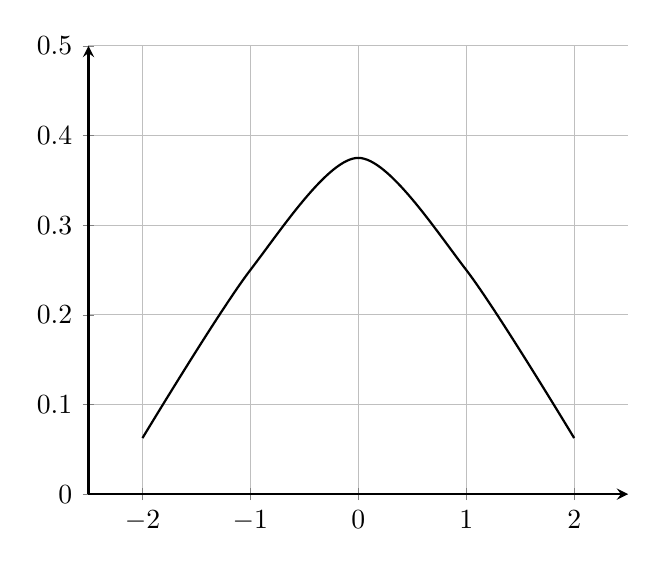
\begin{tikzpicture}
        \begin{axis}[
            axis lines=left,
            xmin=-2.5,
            xmax= 2.5,
            xtick={-3,...,3},
            ymin=0,
            ymax=0.5,
            thick,
            grid=both
            ]
        \addplot[smooth,thick] plot coordinates {
            (-2, 0.0625)
            (-1, 0.2500)
            ( 0, 0.3750)
            ( 1, 0.2500)
            ( 2, 0.0625)
        };
    \end{axis}
\end{tikzpicture}
\end{figure}


% FIGURE: Opponent Processing Diagram
\begin{figure}[h] \label{fig:opp-workflow}
    \centering
    \captionsetup{justification=centering}
    \resizebox{\textwidth}{!}{%
    \begin{tikzpicture}[auto, >=latex']
    % RGB Input
    \draw ( -4.0,  25) node(r)[draw, shape=rectangle, minimum height=1.5cm, minimum width=2cm, align=center] {L};
    \draw (  0.0,  25) node(g)[draw, shape=rectangle, minimum height=1.5cm, minimum width=2cm, align=center] {M};
    \draw (  4.0,  25) node(b)[draw, shape=rectangle, minimum height=1.5cm, minimum width=2cm, align=center] {S};
    % Gaussian Convolutions
    \draw ( -3.0,  18) node(c)[draw, shape=circle, minimum height=5cm, minimum width=5cm, align=center] {};
    \draw (  3.0,  18) node(s)[draw, shape=circle, minimum height=5cm, minimum width=5cm, align=center] {};
    \node at (c.north) [below=0.4cm] {CENTER};
    \node at (c.north) [below=0.9cm] {Convolution};
    \node at (s.north) [below=0.4cm] {SURROUND};
    \node at (s.north) [below=0.9cm] {Convolution};
    % RGB Centers & Surrounds
    \draw ( -9.0,   8) node(rc)[draw, shape=rectangle, minimum height=1cm, align=center] {L Center};
    \draw ( -6.0,  10) node(gc)[draw, shape=rectangle, minimum height=1cm, align=center] {M Center};
    \draw ( -3.0,  12) node(bc)[draw, shape=rectangle, minimum height=1cm, align=center] {S Center};
    \draw (  3.0,  12) node(rs)[draw, shape=rectangle, minimum height=1cm, align=center] {L Surround};
    \draw (  6.0,  10) node(gs)[draw, shape=rectangle, minimum height=1cm, align=center] {M Surround};
    \draw (  9.0,   8) node(bs)[draw, shape=rectangle, minimum height=1cm, align=center] {S Surround};
    % Colors
    \draw (-16.25,  0) node(L)[draw, shape=rectangle, minimum height=1cm, minimum width=2cm, align=center] {Light};
    \draw ( -9.75,  0) node(D)[draw, shape=rectangle, minimum height=1cm, minimum width=2cm, align=center] {Dark};
    \draw ( -3.25,  0) node(R)[draw, shape=rectangle, minimum height=1cm, minimum width=2cm, align=center] {Red};
    \draw (  3.25,  0) node(G)[draw, shape=rectangle, minimum height=1cm, minimum width=2cm, align=center] {Green};
    \draw (  9.75,  0) node(B)[draw, shape=rectangle, minimum height=1cm, minimum width=2cm, align=center] {Blue};
    \draw ( 16.25,  0) node(Y)[draw, shape=rectangle, minimum height=1cm, minimum width=2cm, align=center] {Yellow};
    \node (Lon)  at (L.north) [above left]  {+};
    \node (Don)  at (D.north) [above left]  {+};
    \node (Ron)  at (R.north) [above left]  {+};
    \node (Gon)  at (G.north) [above left]  {+};
    \node (Bon)  at (B.north) [above left]  {+};
    \node (Yon)  at (Y.north) [above left]  {+};
    \node (Loff) at (L.north) [above right] {-};
    \node (Doff) at (D.north) [above right] {-};
    \node (Roff) at (R.north) [above right] {-};
    \node (Goff) at (G.north) [above right] {-};
    \node (Boff) at (B.north) [above right] {-};
    \node (Yoff) at (Y.north) [above right] {-};
    % Paths A
    \draw [->, pomegranate] (r)  to[bend right] (c);
    \draw [->, greensea]    (g)  to             (c);
    \draw [->, peter]       (b)  to             (c);
    \draw [->, pomegranate] (r)  to             (s);
    \draw [->, greensea]    (g)  to             (s);
    \draw [->, peter]       (b)  to[bend left]  (s);
    % Paths B
    \draw [->, pomegranate] (c)  to[bend right] (rc);
    \draw [->, greensea]    (c)  to             (gc);
    \draw [->, peter]       (c)  to             (bc);
    \draw [->, pomegranate] (s)  to             (rs);
    \draw [->, greensea]    (s)  to             (gs);
    \draw [->, peter]       (s)  to[bend left]  (bs);
    % Paths C
    \draw [->, pomegranate] (rc) to[bend right] (Lon);
    \draw [->, greensea]    (gc) to[bend right] (Lon);
    \draw [->, pomegranate] (rs) to             (Loff);
    \draw [->, greensea]    (gs) to             (Loff);
    \draw [->, pomegranate] (rs) to[bend right] (Don);
    \draw [->, greensea]    (gs) to[bend right] (Don);
    \draw [->, pomegranate] (rc) to[bend left]  (Doff);
    \draw [->, greensea]    (gc) to[bend left]  (Doff);
    \draw [->, pomegranate] (rc) to             (Ron);
    \draw [->, greensea]    (gs) to             (Roff);
    \draw [->, greensea]    (gc) to             (Gon);
    \draw [->, pomegranate] (rs) to             (Goff);
    \draw [->, peter]       (bc) to             (Bon);
    \draw [->, greensea]    (gs) to             (Boff);
    \draw [->, pomegranate] (rs) to             (Boff);
    \draw [->, greensea]    (gc) to             (Yon);
    \draw [->, pomegranate] (rc) to             (Yon);
    \draw [->, peter]       (bs) to[bend left]  (Yoff);
    % Example Gaussian Convolutions
    \node[below of=c] {
        \begin{tikzpicture}
            % ON Center
            \draw[gray, very thick] (-1.00, 0.00) .. controls (-0.30, 0.05) .. (-0.05, 2.00);
            \draw[gray, very thick] (-0.05, 2.00) .. controls ( 0.00, 2.10) .. ( 0.05, 2.00);
            \draw[gray, very thick] ( 1.00, 0.00) .. controls ( 0.30, 0.05) .. ( 0.05, 2.00);
            % Reference line & point
            \draw                                                              (-1.50, 0.00) -- ( 1.50, 0.00);
            \filldraw[color=black, fill=gray]                                  ( 0.00, 0.00) circle (2pt);
            % Frame to ensure alignment:
            \draw[opacity=0]                                                   (-3.00, 2.50) rectangle (3.00, -2.50);
        \end{tikzpicture}
    };
    \node[below of=s] {
        \begin{tikzpicture}
            % OFF Surround
            \draw[gray, very thick] (-1.50, 0.00) .. controls (-0.30,-0.20) .. (-0.05,-0.48);
            \draw[gray, very thick] (-0.05,-0.48) .. controls ( 0.00,-0.49) .. ( 0.05,-0.48);
            \draw[gray, very thick] ( 1.50, 0.00) .. controls ( 0.30,-0.20) .. ( 0.05,-0.48);
            % Reference line & point
            \draw                                                              (-1.50, 0.00) -- ( 1.50, 0.00);
            \filldraw[color=black, fill=gray]                                  ( 0.00, 0.00) circle (2pt);
            % Frame to ensure alignment:
            \draw[opacity=0]                                                   (-3.00, 2.50) rectangle (3.00, -2.50);
        \end{tikzpicture}
    };
    % Example Single Opponent Receptive Fields
    \node[below of=L, node distance=1.5in] (Lso) {
        \begin{tikzpicture}
            % ON Center
            \draw[greensea,       dash pattern= on 3pt off 5pt, dash phase=4pt, very thick] (-1.00, 0.00) .. controls (-0.30, 0.05) .. (-0.05, 2.00);
            \draw[greensea,       dash pattern= on 3pt off 5pt, dash phase=4pt, very thick] (-0.05, 2.00) .. controls ( 0.00, 2.10) .. ( 0.05, 2.00);
            \draw[greensea,       dash pattern= on 3pt off 5pt, dash phase=4pt, very thick] ( 1.00, 0.00) .. controls ( 0.30, 0.05) .. ( 0.05, 2.00);
            \draw[pomegranate!80, dash pattern= on 3pt off 5pt, very thick] (-1.00, 0.00) .. controls (-0.30, 0.05) .. (-0.05, 2.00);
            \draw[pomegranate!80, dash pattern= on 3pt off 5pt, very thick] (-0.05, 2.00) .. controls ( 0.00, 2.10) .. ( 0.05, 2.00);
            \draw[pomegranate!80, dash pattern= on 3pt off 5pt, very thick] ( 1.00, 0.00) .. controls ( 0.30, 0.05) .. ( 0.05, 2.00)
                 node[color=black, anchor=south west] {$L^+M^+$};
            % OFF Surround
            \draw[pomegranate!80, dash pattern= on 3pt off 5pt, dash phase=4pt, very thick] (-1.50, 0.00) .. controls (-0.30,-0.20) .. (-0.05,-0.48);
            \draw[pomegranate!80, dash pattern= on 3pt off 5pt, dash phase=4pt, very thick] (-0.05,-0.48) .. controls ( 0.00,-0.49) .. ( 0.05,-0.48);
            \draw[pomegranate!80, dash pattern= on 3pt off 5pt, dash phase=4pt, very thick] ( 1.50, 0.00) .. controls ( 0.30,-0.20) .. ( 0.05,-0.48);
            \draw[greensea,       dash pattern= on 3pt off 5pt, very thick] (-1.50, 0.00) .. controls (-0.30,-0.20) .. (-0.05,-0.48);
            \draw[greensea,       dash pattern= on 3pt off 5pt, very thick] (-0.05,-0.48) .. controls ( 0.00,-0.49) .. ( 0.05,-0.48);
            \draw[greensea,       dash pattern= on 3pt off 5pt, very thick] ( 1.50, 0.00) .. controls ( 0.30,-0.20) .. ( 0.05,-0.48)
                 node[color=black, anchor=north west] {$L^-M^-$};
            % Reference line & point
            \draw                                                             (-1.50, 0.00) -- ( 1.50, 0.00);
            \filldraw[color=black, fill=gray]                                 ( 0.00, 0.00) circle (2pt);
            % Frame to ensure alignment:
            \draw[opacity=0]                                                  (-3.00, 2.50) rectangle (3.00, -2.50);
        \end{tikzpicture}
    };
    \node[below of=D, node distance=1.5in] (Dso) {
        \begin{tikzpicture}
            \begin{scope}[rotate=180]
            % OFF Center
            \draw[greensea,       dash pattern= on 3pt off 5pt, dash phase=4pt, very thick] (-1.00, 0.00) .. controls (-0.30, 0.05) .. (-0.05, 2.00);
            \draw[greensea,       dash pattern= on 3pt off 5pt, dash phase=4pt, very thick] (-0.05, 2.00) .. controls ( 0.00, 2.10) .. ( 0.05, 2.00);
            \draw[greensea,       dash pattern= on 3pt off 5pt, dash phase=4pt, very thick] ( 1.00, 0.00) .. controls ( 0.30, 0.05) .. ( 0.05, 2.00);
            \draw[pomegranate!80, dash pattern= on 3pt off 5pt, very thick] (-1.00, 0.00) .. controls (-0.30, 0.05) .. (-0.05, 2.00);
            \draw[pomegranate!80, dash pattern= on 3pt off 5pt, very thick] (-0.05, 2.00) .. controls ( 0.00, 2.10) .. ( 0.05, 2.00);
            \draw[pomegranate!80, dash pattern= on 3pt off 5pt, very thick] ( 1.00, 0.00) .. controls ( 0.30, 0.05) .. ( 0.05, 2.00)
                 node[color=black, anchor=north west] {$L^-M^-$};
            % ON Surround
            \draw[pomegranate!80, dash pattern= on 3pt off 5pt, dash phase=4pt, very thick] (-1.50, 0.00) .. controls (-0.30,-0.20) .. (-0.05,-0.48);
            \draw[pomegranate!80, dash pattern= on 3pt off 5pt, dash phase=4pt, very thick] (-0.05,-0.48) .. controls ( 0.00,-0.49) .. ( 0.05,-0.48);
            \draw[pomegranate!80, dash pattern= on 3pt off 5pt, dash phase=4pt, very thick] ( 1.50, 0.00) .. controls ( 0.30,-0.20) .. ( 0.05,-0.48);
            \draw[greensea,       dash pattern= on 3pt off 5pt, very thick] (-1.50, 0.00) .. controls (-0.30,-0.20) .. (-0.05,-0.48);
            \draw[greensea,       dash pattern= on 3pt off 5pt, very thick] (-0.05,-0.48) .. controls ( 0.00,-0.49) .. ( 0.05,-0.48);
            \draw[greensea,       dash pattern= on 3pt off 5pt, very thick] ( 1.50, 0.00) .. controls ( 0.30,-0.20) .. ( 0.05,-0.48)
                 node[color=black, anchor=south west] {$L^+M^+$};
            % Reference line & point
            \draw                                                             (-1.50, 0.00) -- ( 1.50, 0.00);
            \filldraw[color=black, fill=gray]                                 ( 0.00, 0.00) circle (2pt);
            % Frame to ensure alignment:
            \draw[opacity=0]                                                  (-3.00, 2.50) rectangle (3.00, -2.50);
            \end{scope}
        \end{tikzpicture}
    };
    \node[below of=R, node distance=1.5in] (Rso) {
        \begin{tikzpicture}
            % ON Center
            \draw[pomegranate!80, very thick] (-1.00, 0.00) .. controls (-0.30, 0.05) .. (-0.05, 2.00);
            \draw[pomegranate!80, very thick] (-0.05, 2.00) .. controls ( 0.00, 2.10) .. ( 0.05, 2.00);
            \draw[pomegranate!80, very thick] ( 1.00, 0.00) .. controls ( 0.30, 0.05) .. ( 0.05, 2.00)
                 node[color=black, anchor=south west] {$L^+$};
            % OFF Surround
            \draw[greensea,       very thick] (-1.50, 0.00) .. controls (-0.30,-0.20) .. (-0.05,-0.48);
            \draw[greensea,       very thick] (-0.05,-0.48) .. controls ( 0.00,-0.49) .. ( 0.05,-0.48);
            \draw[greensea,       very thick] ( 1.50, 0.00) .. controls ( 0.30,-0.20) .. ( 0.05,-0.48)
                 node[color=black, anchor=north west] {$M^-$};
            % Reference line & point
            \draw                                                             (-1.50, 0.00) -- ( 1.50, 0.00);
            \filldraw[color=black, fill=gray]                                 ( 0.00, 0.00) circle (2pt);
            % Frame to ensure alignment:
            \draw[opacity=0]                                                  (-3.00, 2.50) rectangle (3.00, -2.50);
        \end{tikzpicture}
    };
    \node[below of=G, node distance=1.5in] (Gso) {
        \begin{tikzpicture}
            % ON Center
            \draw[greensea,       very thick] (-1.00, 0.00) .. controls (-0.30, 0.05) .. (-0.05, 2.00);
            \draw[greensea,       very thick] (-0.05, 2.00) .. controls ( 0.00, 2.10) .. ( 0.05, 2.00);
            \draw[greensea,       very thick] ( 1.00, 0.00) .. controls ( 0.30, 0.05) .. ( 0.05, 2.00)
                 node[color=black, anchor=south west] {$M^+$};
            % OFF Surround
            \draw[pomegranate!80, very thick] (-1.50, 0.00) .. controls (-0.30,-0.20) .. (-0.05,-0.48);
            \draw[pomegranate!80, very thick] (-0.05,-0.48) .. controls ( 0.00,-0.49) .. ( 0.05,-0.48);
            \draw[pomegranate!80, very thick] ( 1.50, 0.00) .. controls ( 0.30,-0.20) .. ( 0.05,-0.48)
                 node[color=black, anchor=north west] {$L^-$};
            % Reference line & point
            \draw                                                             (-1.50, 0.00) -- ( 1.50, 0.00);
            \filldraw[color=black, fill=gray]                                 ( 0.00, 0.00) circle (2pt);
            % Frame to ensure alignment:
            \draw[opacity=0]                                                  (-3.00, 2.50) rectangle (3.00, -2.50);
        \end{tikzpicture}
    };
    \node[below of=B, node distance=1.5in] (Bso) {
        \begin{tikzpicture}
            % ON Center
            \draw[peter,          very thick] (-1.00, 0.00) .. controls (-0.30, 0.05) .. (-0.05, 2.00);
            \draw[peter,          very thick] (-0.05, 2.00) .. controls ( 0.00, 2.10) .. ( 0.05, 2.00);
            \draw[peter,          very thick] ( 1.00, 0.00) .. controls ( 0.30, 0.05) .. ( 0.05, 2.00)
                 node[color=black, anchor=south west] {$S^+$};
            % OFF Surround
            \draw[pomegranate!80, dash pattern= on 3pt off 5pt, dash phase=4pt, very thick] (-1.50, 0.00) .. controls (-0.30,-0.20) .. (-0.05,-0.48);
            \draw[pomegranate!80, dash pattern= on 3pt off 5pt, dash phase=4pt, very thick] (-0.05,-0.48) .. controls ( 0.00,-0.49) .. ( 0.05,-0.48);
            \draw[pomegranate!80, dash pattern= on 3pt off 5pt, dash phase=4pt, very thick] ( 1.50, 0.00) .. controls ( 0.30,-0.20) .. ( 0.05,-0.48);
            \draw[greensea,       dash pattern= on 3pt off 5pt, very thick] (-1.50, 0.00) .. controls (-0.30,-0.20) .. (-0.05,-0.48);
            \draw[greensea,       dash pattern= on 3pt off 5pt, very thick] (-0.05,-0.48) .. controls ( 0.00,-0.49) .. ( 0.05,-0.48);
            \draw[greensea,       dash pattern= on 3pt off 5pt, very thick] ( 1.50, 0.00) .. controls ( 0.30,-0.20) .. ( 0.05,-0.48)
                 node[color=black, anchor=north west] {$L^-M^-$};
            % Reference line & point
            \draw                                                             (-1.50, 0.00) -- ( 1.50, 0.00);
            \filldraw[color=black, fill=gray]                                 ( 0.00, 0.00) circle (2pt);
            % Frame to ensure alignment:
            \draw[opacity=0]                                                  (-3.00, 2.50) rectangle (3.00, -2.50);
        \end{tikzpicture}
    };
    \node[below of=Y, node distance=1.5in] (Yso) {
        \begin{tikzpicture}
            % ON Center
            \draw[greensea,       dash pattern= on 3pt off 5pt, dash phase=4pt, very thick] (-1.00, 0.00) .. controls (-0.30, 0.05) .. (-0.05, 2.00);
            \draw[greensea,       dash pattern= on 3pt off 5pt, dash phase=4pt, very thick] (-0.05, 2.00) .. controls ( 0.00, 2.10) .. ( 0.05, 2.00);
            \draw[greensea,       dash pattern= on 3pt off 5pt, dash phase=4pt, very thick] ( 1.00, 0.00) .. controls ( 0.30, 0.05) .. ( 0.05, 2.00);
            \draw[pomegranate!80, dash pattern= on 3pt off 5pt, very thick] (-1.00, 0.00) .. controls (-0.30, 0.05) .. (-0.05, 2.00);
            \draw[pomegranate!80, dash pattern= on 3pt off 5pt, very thick] (-0.05, 2.00) .. controls ( 0.00, 2.10) .. ( 0.05, 2.00);
            \draw[pomegranate!80, dash pattern= on 3pt off 5pt, very thick] ( 1.00, 0.00) .. controls ( 0.30, 0.05) .. ( 0.05, 2.00)
                 node[color=black, anchor=south west] {$L^+M^+$};
            % OFF Surround
            \draw[peter,          very thick] (-1.50, 0.00) .. controls (-0.30,-0.20) .. (-0.05,-0.48);
            \draw[peter,          very thick] (-0.05,-0.48) .. controls ( 0.00,-0.49) .. ( 0.05,-0.48);
            \draw[peter,          very thick] ( 1.50, 0.00) .. controls ( 0.30,-0.20) .. ( 0.05,-0.48)
                 node[color=black, anchor=north west] {$S^-$};
            % Reference line & point
            \draw                                                             (-1.50, 0.00) -- ( 1.50, 0.00);
            \filldraw[color=black, fill=gray]                                 ( 0.00, 0.00) circle (2pt);
            % Frame to ensure alignment:
            \draw[opacity=0]                                                  (-3.00, 2.50) rectangle (3.00, -2.50);
        \end{tikzpicture}
    };
    \end{tikzpicture}
    }
    \caption{Diagram of \textit{Opponent Processing of Receptive Fields} workflow. The L, M, and S channels are convoluted with center and surround gaussians and then combined to build opponent colors, here exemplified by single-opponent cell receptive fields.}
\end{figure}


% FIGURE: Colored Double Opponent Receptive Fields
\begin{figure}
    \centering
    \captionsetup{justification=centering}
    % 3 SUBFIGURES: Cross sections of single-opponent receptive fields
    \begin{subfigure}{0.3\textwidth}
        \centering
        \resizebox{\textwidth}{!}{%
        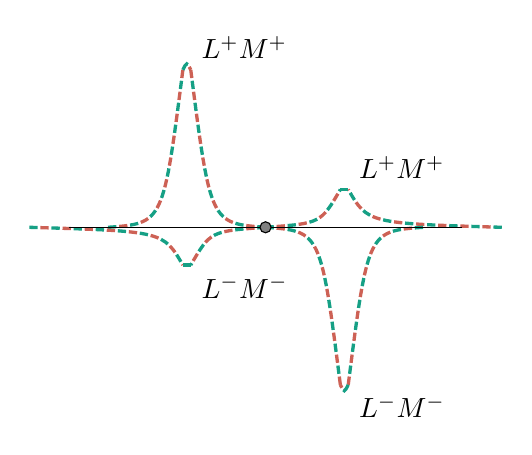
\begin{tikzpicture}
            % ON Center
            \draw[pomegranate!80, dash pattern= on 3pt off 5pt, dash phase=4pt, very thick] (-2.00, 0.00) .. controls (-1.30, 0.05) .. (-1.05, 2.00);
            \draw[pomegranate!80, dash pattern= on 3pt off 5pt, dash phase=4pt, very thick] (-1.05, 2.00) .. controls (-1.00, 2.10) .. (-0.95, 2.00);
            \draw[pomegranate!80, dash pattern= on 3pt off 5pt, dash phase=4pt, very thick] ( 0.00, 0.00) .. controls (-0.70, 0.05) .. (-0.95, 2.00);
            \draw[greensea,       dash pattern= on 3pt off 5pt, very thick]                 (-2.00, 0.00) .. controls (-1.30, 0.05) .. (-1.05, 2.00);
            \draw[greensea,       dash pattern= on 3pt off 5pt, very thick]                 (-1.05, 2.00) .. controls (-1.00, 2.10) .. (-0.95, 2.00);
            \draw[greensea,       dash pattern= on 3pt off 5pt, very thick]                 ( 0.00, 0.00) .. controls (-0.70, 0.05) .. (-0.95, 2.00)
                 node[color=black, anchor=south west] {$L^+M^+$};
            % OFF Surround
            \draw[pomegranate!80, dash pattern= on 3pt off 5pt, dash phase=4pt, very thick] (-3.00, 0.00) .. controls (-1.30,-0.05) .. (-1.05,-0.48);
            \draw[pomegranate!80, dash pattern= on 3pt off 5pt, dash phase=4pt, very thick] (-1.05,-0.48) .. controls (-1.00,-0.49) .. (-0.95,-0.48);
            \draw[pomegranate!80, dash pattern= on 3pt off 5pt, dash phase=4pt, very thick] ( 0.00, 0.00) .. controls (-0.70,-0.05) .. (-0.95,-0.48);
            \draw[greensea,       dash pattern= on 3pt off 5pt, very thick]                 (-3.00, 0.00) .. controls (-1.30,-0.05) .. (-1.05,-0.48);
            \draw[greensea,       dash pattern= on 3pt off 5pt, very thick]                 (-1.05,-0.48) .. controls (-1.00,-0.49) .. (-0.95,-0.48);
            \draw[greensea,       dash pattern= on 3pt off 5pt, very thick]                 ( 0.00, 0.00) .. controls (-0.70,-0.05) .. (-0.95,-0.48)
                 node[color=black, anchor=north west] {$L^-M^-$};
            % ON Center
            \draw[pomegranate!80, dash pattern= on 3pt off 5pt, dash phase=4pt, very thick] ( 0.00, 0.00) .. controls ( 0.70, 0.05) .. ( 0.95, 0.48);
            \draw[pomegranate!80, dash pattern= on 3pt off 5pt, dash phase=4pt, very thick] ( 1.05, 0.48) .. controls ( 1.00, 0.49) .. ( 0.95, 0.48);
            \draw[pomegranate!80, dash pattern= on 3pt off 5pt, dash phase=4pt, very thick] ( 3.00, 0.00) .. controls ( 1.30, 0.05) .. ( 1.05, 0.48);
            \draw[greensea,       dash pattern= on 3pt off 5pt, very thick]                 ( 0.00, 0.00) .. controls ( 0.70, 0.05) .. ( 0.95, 0.48);
            \draw[greensea,       dash pattern= on 3pt off 5pt, very thick]                 ( 1.05, 0.48) .. controls ( 1.00, 0.49) .. ( 0.95, 0.48);
            \draw[greensea,       dash pattern= on 3pt off 5pt, very thick]                 ( 3.00, 0.00) .. controls ( 1.30, 0.05) .. ( 1.05, 0.48)
                 node[color=black, anchor=south west] {$L^+M^+$};
            % OFF Surround
            \draw[pomegranate!80, dash pattern= on 3pt off 5pt, dash phase=4pt, very thick] ( 0.00, 0.00) .. controls ( 0.70,-0.05) .. ( 0.95,-2.00);
            \draw[pomegranate!80, dash pattern= on 3pt off 5pt, dash phase=4pt, very thick] ( 1.05,-2.00) .. controls ( 1.00,-2.10) .. ( 0.95,-2.00);
            \draw[pomegranate!80, dash pattern= on 3pt off 5pt, dash phase=4pt, very thick] ( 2.00, 0.00) .. controls ( 1.30,-0.05) .. ( 1.05,-2.00);
            \draw[greensea,       dash pattern= on 3pt off 5pt, very thick]                 ( 0.00, 0.00) .. controls ( 0.70,-0.05) .. ( 0.95,-2.00);
            \draw[greensea,       dash pattern= on 3pt off 5pt, very thick]                 ( 1.05,-2.00) .. controls ( 1.00,-2.10) .. ( 0.95,-2.00);
            \draw[greensea,       dash pattern= on 3pt off 5pt, very thick]                 ( 2.00, 0.00) .. controls ( 1.30,-0.05) .. ( 1.05,-2.00)
                 node[color=black, anchor=north west] {$L^-M^-$};
            % Reference line & point
            \draw                                                             (-2.50, 0.00) -- ( 2.50, 0.00);
            \filldraw[color=black, fill=gray]                                 ( 0.00, 0.00) circle (2pt);
            % Frame to ensure alignment:
            \draw[opacity=0]                                                  (-3.00, 2.50) rectangle (3.00, -2.50);
        \end{tikzpicture}
    }
    \caption{Light DO \\ Receptive Field}
    \end{subfigure}%
    \begin{subfigure}{0.3\textwidth}
        \centering
        \resizebox{\textwidth}{!}{%
        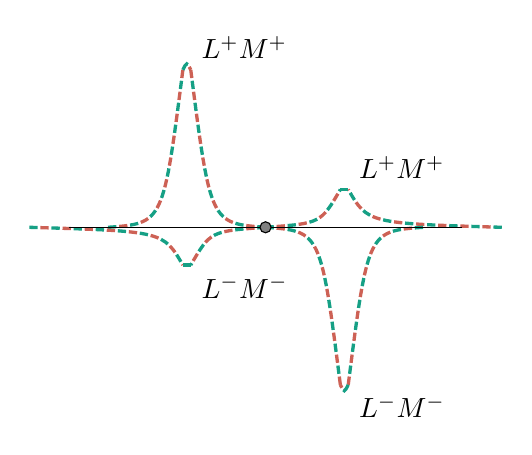
\begin{tikzpicture}
            % ON Center
            \draw[pomegranate!80, dash pattern= on 3pt off 5pt, dash phase=4pt, very thick] (-2.00, 0.00) .. controls (-1.30, 0.05) .. (-1.05, 2.00);
            \draw[pomegranate!80, dash pattern= on 3pt off 5pt, dash phase=4pt, very thick] (-1.05, 2.00) .. controls (-1.00, 2.10) .. (-0.95, 2.00);
            \draw[pomegranate!80, dash pattern= on 3pt off 5pt, dash phase=4pt, very thick] ( 0.00, 0.00) .. controls (-0.70, 0.05) .. (-0.95, 2.00);
            \draw[greensea,       dash pattern= on 3pt off 5pt, very thick]                 (-2.00, 0.00) .. controls (-1.30, 0.05) .. (-1.05, 2.00);
            \draw[greensea,       dash pattern= on 3pt off 5pt, very thick]                 (-1.05, 2.00) .. controls (-1.00, 2.10) .. (-0.95, 2.00);
            \draw[greensea,       dash pattern= on 3pt off 5pt, very thick]                 ( 0.00, 0.00) .. controls (-0.70, 0.05) .. (-0.95, 2.00)
                 node[color=black, anchor=south west] {$L^+M^+$};
            % OFF Surround
            \draw[pomegranate!80, dash pattern= on 3pt off 5pt, dash phase=4pt, very thick] (-3.00, 0.00) .. controls (-1.30,-0.05) .. (-1.05,-0.48);
            \draw[pomegranate!80, dash pattern= on 3pt off 5pt, dash phase=4pt, very thick] (-1.05,-0.48) .. controls (-1.00,-0.49) .. (-0.95,-0.48);
            \draw[pomegranate!80, dash pattern= on 3pt off 5pt, dash phase=4pt, very thick] ( 0.00, 0.00) .. controls (-0.70,-0.05) .. (-0.95,-0.48);
            \draw[greensea,       dash pattern= on 3pt off 5pt, very thick]                 (-3.00, 0.00) .. controls (-1.30,-0.05) .. (-1.05,-0.48);
            \draw[greensea,       dash pattern= on 3pt off 5pt, very thick]                 (-1.05,-0.48) .. controls (-1.00,-0.49) .. (-0.95,-0.48);
            \draw[greensea,       dash pattern= on 3pt off 5pt, very thick]                 ( 0.00, 0.00) .. controls (-0.70,-0.05) .. (-0.95,-0.48)
                 node[color=black, anchor=north west] {$L^-M^-$};
            % ON Center
            \draw[pomegranate!80, dash pattern= on 3pt off 5pt, dash phase=4pt, very thick] ( 0.00, 0.00) .. controls ( 0.70, 0.05) .. ( 0.95, 0.48);
            \draw[pomegranate!80, dash pattern= on 3pt off 5pt, dash phase=4pt, very thick] ( 1.05, 0.48) .. controls ( 1.00, 0.49) .. ( 0.95, 0.48);
            \draw[pomegranate!80, dash pattern= on 3pt off 5pt, dash phase=4pt, very thick] ( 3.00, 0.00) .. controls ( 1.30, 0.05) .. ( 1.05, 0.48);
            \draw[greensea,       dash pattern= on 3pt off 5pt, very thick]                 ( 0.00, 0.00) .. controls ( 0.70, 0.05) .. ( 0.95, 0.48);
            \draw[greensea,       dash pattern= on 3pt off 5pt, very thick]                 ( 1.05, 0.48) .. controls ( 1.00, 0.49) .. ( 0.95, 0.48);
            \draw[greensea,       dash pattern= on 3pt off 5pt, very thick]                 ( 3.00, 0.00) .. controls ( 1.30, 0.05) .. ( 1.05, 0.48)
                 node[color=black, anchor=south west] {$L^+M^+$};
            % OFF Surround
            \draw[pomegranate!80, dash pattern= on 3pt off 5pt, dash phase=4pt, very thick] ( 0.00, 0.00) .. controls ( 0.70,-0.05) .. ( 0.95,-2.00);
            \draw[pomegranate!80, dash pattern= on 3pt off 5pt, dash phase=4pt, very thick] ( 1.05,-2.00) .. controls ( 1.00,-2.10) .. ( 0.95,-2.00);
            \draw[pomegranate!80, dash pattern= on 3pt off 5pt, dash phase=4pt, very thick] ( 2.00, 0.00) .. controls ( 1.30,-0.05) .. ( 1.05,-2.00);
            \draw[greensea,       dash pattern= on 3pt off 5pt, very thick]                 ( 0.00, 0.00) .. controls ( 0.70,-0.05) .. ( 0.95,-2.00);
            \draw[greensea,       dash pattern= on 3pt off 5pt, very thick]                 ( 1.05,-2.00) .. controls ( 1.00,-2.10) .. ( 0.95,-2.00);
            \draw[greensea,       dash pattern= on 3pt off 5pt, very thick]                 ( 2.00, 0.00) .. controls ( 1.30,-0.05) .. ( 1.05,-2.00)
                 node[color=black, anchor=north west] {$L^-M^-$};
            % Reference line & point
            \draw                                                             (-2.50, 0.00) -- ( 2.50, 0.00);
            \filldraw[color=black, fill=gray]                                 ( 0.00, 0.00) circle (2pt);
            % Frame to ensure alignment:
            \draw[opacity=0]                                                  (-3.00, 2.50) rectangle (3.00, -2.50);
        \end{tikzpicture}
    }
    \caption{Dark DO \\ Receptive Field}
    \end{subfigure}%
    \par \bigskip
    \begin{subfigure}{0.3\textwidth}
        \centering
        \resizebox{\textwidth}{!}{%
        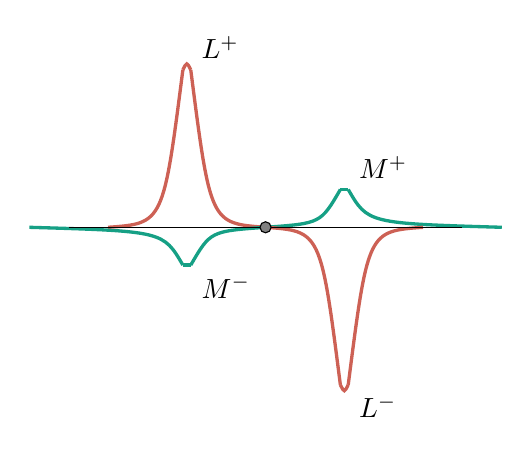
\begin{tikzpicture}
            % ON Center
            \draw[pomegranate!80, very thick] (-2.00, 0.00) .. controls (-1.30, 0.05) .. (-1.05, 2.00);
            \draw[pomegranate!80, very thick] (-1.05, 2.00) .. controls (-1.00, 2.10) .. (-0.95, 2.00);
            \draw[pomegranate!80, very thick] ( 0.00, 0.00) .. controls (-0.70, 0.05) .. (-0.95, 2.00)
                 node[color=black, anchor=south west] {$L^+$};
            % OFF Surround
            \draw[greensea,       very thick] (-3.00, 0.00) .. controls (-1.30,-0.05) .. (-1.05,-0.48);
            \draw[greensea,       very thick] (-1.05,-0.48) .. controls (-1.00,-0.49) .. (-0.95,-0.48);
            \draw[greensea,       very thick] ( 0.00, 0.00) .. controls (-0.70,-0.05) .. (-0.95,-0.48)
                 node[color=black, anchor=north west] {$M^-$};
            % ON Center
            \draw[greensea,       very thick] ( 0.00, 0.00) .. controls ( 0.70, 0.05) .. ( 0.95, 0.48);
            \draw[greensea,       very thick] ( 1.05, 0.48) .. controls ( 1.00, 0.49) .. ( 0.95, 0.48);
            \draw[greensea,       very thick] ( 3.00, 0.00) .. controls ( 1.30, 0.05) .. ( 1.05, 0.48)
                 node[color=black, anchor=south west] {$M^+$};
            % OFF Surround
            \draw[pomegranate!80, very thick] ( 0.00, 0.00) .. controls ( 0.70,-0.05) .. ( 0.95,-2.00);
            \draw[pomegranate!80, very thick] ( 1.05,-2.00) .. controls ( 1.00,-2.10) .. ( 0.95,-2.00);
            \draw[pomegranate!80, very thick] ( 2.00, 0.00) .. controls ( 1.30,-0.05) .. ( 1.05,-2.00)
                 node[color=black, anchor=north west] {$L^-$};
            % Reference line & point
            \draw                                                             (-2.50, 0.00) -- ( 2.50, 0.00);
            \filldraw[color=black, fill=gray]                                 ( 0.00, 0.00) circle (2pt);
            % Frame to ensure alignment:
            \draw[opacity=0]                                                  (-3.00, 2.50) rectangle (3.00, -2.50);
        \end{tikzpicture}
    }
    \caption{Red DO \\ Receptive Field}
    \end{subfigure}%
    \begin{subfigure}{0.3\textwidth}
        \centering
        \resizebox{\textwidth}{!}{%
        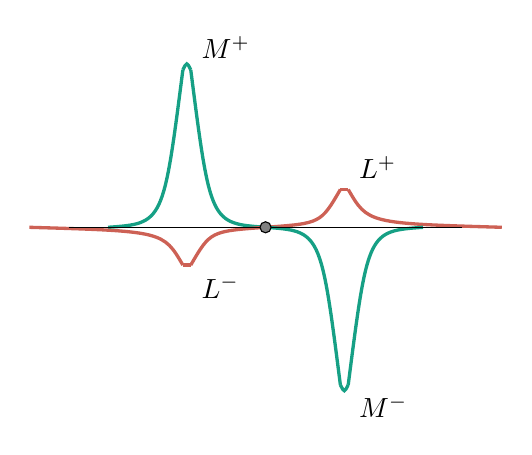
\begin{tikzpicture}
            % ON Center
            \draw[greensea, very thick] (-2.00, 0.00) .. controls (-1.30, 0.05) .. (-1.05, 2.00);
            \draw[greensea, very thick] (-1.05, 2.00) .. controls (-1.00, 2.10) .. (-0.95, 2.00);
            \draw[greensea, very thick] ( 0.00, 0.00) .. controls (-0.70, 0.05) .. (-0.95, 2.00)
                 node[color=black, anchor=south west] {$M^+$};
            % OFF Surround
            \draw[pomegranate!80,       very thick] (-3.00, 0.00) .. controls (-1.30,-0.05) .. (-1.05,-0.48);
            \draw[pomegranate!80,       very thick] (-1.05,-0.48) .. controls (-1.00,-0.49) .. (-0.95,-0.48);
            \draw[pomegranate!80,       very thick] ( 0.00, 0.00) .. controls (-0.70,-0.05) .. (-0.95,-0.48)
                 node[color=black, anchor=north west] {$L^-$};
            % ON Center
            \draw[pomegranate!80,       very thick] ( 0.00, 0.00) .. controls ( 0.70, 0.05) .. ( 0.95, 0.48);
            \draw[pomegranate!80,       very thick] ( 1.05, 0.48) .. controls ( 1.00, 0.49) .. ( 0.95, 0.48);
            \draw[pomegranate!80,       very thick] ( 3.00, 0.00) .. controls ( 1.30, 0.05) .. ( 1.05, 0.48)
                 node[color=black, anchor=south west] {$L^+$};
            % OFF Surround
            \draw[greensea, very thick] ( 0.00, 0.00) .. controls ( 0.70,-0.05) .. ( 0.95,-2.00);
            \draw[greensea, very thick] ( 1.05,-2.00) .. controls ( 1.00,-2.10) .. ( 0.95,-2.00);
            \draw[greensea, very thick] ( 2.00, 0.00) .. controls ( 1.30,-0.05) .. ( 1.05,-2.00)
                 node[color=black, anchor=north west] {$M^-$};
            % Reference line & point
            \draw                                                             (-2.50, 0.00) -- ( 2.50, 0.00);
            \filldraw[color=black, fill=gray]                                 ( 0.00, 0.00) circle (2pt);
            % Frame to ensure alignment:
            \draw[opacity=0]                                                  (-3.00, 2.50) rectangle (3.00, -2.50);
        \end{tikzpicture}
    }
    \caption{Green DO \\ Receptive Field}
    \end{subfigure}%
    \par \bigskip
    \begin{subfigure}{0.3\textwidth}
        \centering
        \resizebox{\textwidth}{!}{%
        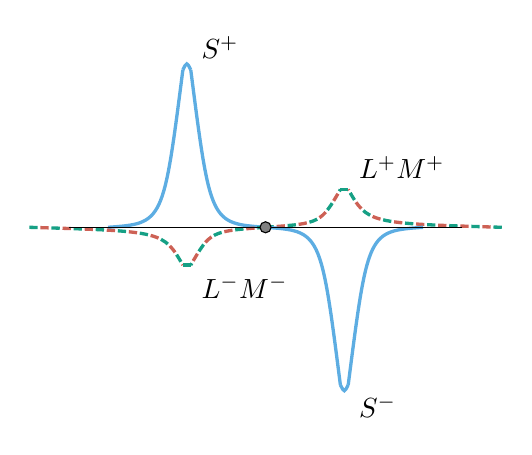
\begin{tikzpicture}
            % ON Center
            \draw[color=peter!80, very thick] (-2.00, 0.00) .. controls (-1.30, 0.05) .. (-1.05, 2.00);
            \draw[color=peter!80, very thick] (-1.05, 2.00) .. controls (-1.00, 2.10) .. (-0.95, 2.00);
            \draw[color=peter!80, very thick] ( 0.00, 0.00) .. controls (-0.70, 0.05) .. (-0.95, 2.00)
                 node[color=black, anchor=south west] {$S^+$};
            % OFF Surround
            \draw[pomegranate!80, dash pattern= on 3pt off 5pt, dash phase=4pt, very thick] (-3.00, 0.00) .. controls (-1.30,-0.05) .. (-1.05,-0.48);
            \draw[pomegranate!80, dash pattern= on 3pt off 5pt, dash phase=4pt, very thick] (-1.05,-0.48) .. controls (-1.00,-0.49) .. (-0.95,-0.48);
            \draw[pomegranate!80, dash pattern= on 3pt off 5pt, dash phase=4pt, very thick] ( 0.00, 0.00) .. controls (-0.70,-0.05) .. (-0.95,-0.48);
            \draw[greensea,       dash pattern= on 3pt off 5pt, very thick] (-3.00, 0.00) .. controls (-1.30,-0.05) .. (-1.05,-0.48);
            \draw[greensea,       dash pattern= on 3pt off 5pt, very thick] (-1.05,-0.48) .. controls (-1.00,-0.49) .. (-0.95,-0.48);
            \draw[greensea,       dash pattern= on 3pt off 5pt, very thick] ( 0.00, 0.00) .. controls (-0.70,-0.05) .. (-0.95,-0.48)
                 node[color=black, anchor=north west] {$L^-M^-$};
            % ON Center
            \draw[pomegranate!80, dash pattern= on 3pt off 5pt, dash phase=4pt, very thick] ( 0.00, 0.00) .. controls ( 0.70, 0.05) .. ( 0.95, 0.48);
            \draw[pomegranate!80, dash pattern= on 3pt off 5pt, dash phase=4pt, very thick] ( 1.05, 0.48) .. controls ( 1.00, 0.49) .. ( 0.95, 0.48);
            \draw[pomegranate!80, dash pattern= on 3pt off 5pt, dash phase=4pt, very thick] ( 3.00, 0.00) .. controls ( 1.30, 0.05) .. ( 1.05, 0.48);
            \draw[greensea,       dash pattern= on 3pt off 5pt, very thick] ( 0.00, 0.00) .. controls ( 0.70, 0.05) .. ( 0.95, 0.48);
            \draw[greensea,       dash pattern= on 3pt off 5pt, very thick] ( 1.05, 0.48) .. controls ( 1.00, 0.49) .. ( 0.95, 0.48);
            \draw[greensea,       dash pattern= on 3pt off 5pt, very thick] ( 3.00, 0.00) .. controls ( 1.30, 0.05) .. ( 1.05, 0.48)
                 node[color=black, anchor=south west] {$L^+M^+$};
            % OFF Surround
            \draw[color=peter!80, very thick] ( 0.00, 0.00) .. controls ( 0.70,-0.05) .. ( 0.95,-2.00);
            \draw[color=peter!80, very thick] ( 1.05,-2.00) .. controls ( 1.00,-2.10) .. ( 0.95,-2.00);
            \draw[color=peter!80, very thick] ( 2.00, 0.00) .. controls ( 1.30,-0.05) .. ( 1.05,-2.00)
                 node[color=black, anchor=north west] {$S^-$};
            % Reference line & point
            \draw                                                             (-2.50, 0.00) -- ( 2.50, 0.00);
            \filldraw[color=black, fill=gray]                                 ( 0.00, 0.00) circle (2pt);
            % Frame to ensure alignment:
            \draw[opacity=0]                                                  (-3.00, 2.50) rectangle (3.00, -2.50);
        \end{tikzpicture}
    }
    \caption{Blue DO \\ Receptive Field}
    \end{subfigure}%
    \begin{subfigure}{0.3\textwidth}
        \centering
        \resizebox{\textwidth}{!}{%
        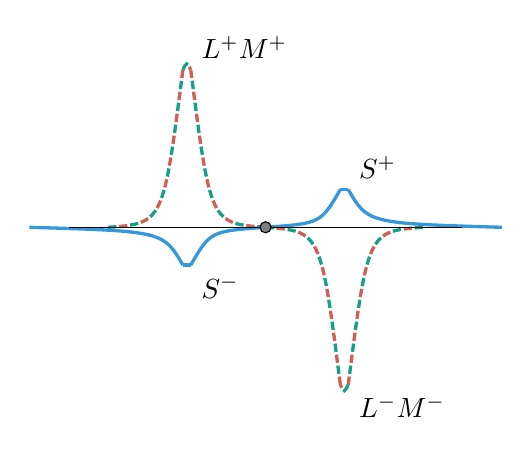
\begin{tikzpicture}
            % ON Center
            \draw[pomegranate!80, dash pattern= on 3pt off 5pt, dash phase=4pt, very thick] (-2.00, 0.00) .. controls (-1.30, 0.05) .. (-1.05, 2.00);
            \draw[pomegranate!80, dash pattern= on 3pt off 5pt, dash phase=4pt, very thick] (-1.05, 2.00) .. controls (-1.00, 2.10) .. (-0.95, 2.00);
            \draw[pomegranate!80, dash pattern= on 3pt off 5pt, dash phase=4pt, very thick] ( 0.00, 0.00) .. controls (-0.70, 0.05) .. (-0.95, 2.00);
            \draw[greensea,       dash pattern= on 3pt off 5pt, very thick]                 (-2.00, 0.00) .. controls (-1.30, 0.05) .. (-1.05, 2.00);
            \draw[greensea,       dash pattern= on 3pt off 5pt, very thick]                 (-1.05, 2.00) .. controls (-1.00, 2.10) .. (-0.95, 2.00);
            \draw[greensea,       dash pattern= on 3pt off 5pt, very thick]                 ( 0.00, 0.00) .. controls (-0.70, 0.05) .. (-0.95, 2.00)
                 node[color=black, anchor=south west] {$L^+M^+$};
            % OFF Surround
            \draw[color=peter,       very thick] (-3.00, 0.00) .. controls (-1.30,-0.05) .. (-1.05,-0.48);
            \draw[color=peter,       very thick] (-1.05,-0.48) .. controls (-1.00,-0.49) .. (-0.95,-0.48);
            \draw[color=peter,       very thick] ( 0.00, 0.00) .. controls (-0.70,-0.05) .. (-0.95,-0.48)
                 node[color=black, anchor=north west] {$S^-$};
            % ON Center
            \draw[color=peter,       very thick] ( 0.00, 0.00) .. controls ( 0.70, 0.05) .. ( 0.95, 0.48);
            \draw[color=peter,       very thick] ( 1.05, 0.48) .. controls ( 1.00, 0.49) .. ( 0.95, 0.48);
            \draw[color=peter,       very thick] ( 3.00, 0.00) .. controls ( 1.30, 0.05) .. ( 1.05, 0.48)
                 node[color=black, anchor=south west] {$S^+$};
            % OFF Surround
            \draw[pomegranate!80, dash pattern= on 3pt off 5pt, dash phase=4pt, very thick] ( 0.00, 0.00) .. controls ( 0.70,-0.05) .. ( 0.95,-2.00);
            \draw[pomegranate!80, dash pattern= on 3pt off 5pt, dash phase=4pt, very thick] ( 1.05,-2.00) .. controls ( 1.00,-2.10) .. ( 0.95,-2.00);
            \draw[pomegranate!80, dash pattern= on 3pt off 5pt, dash phase=4pt, very thick] ( 2.00, 0.00) .. controls ( 1.30,-0.05) .. ( 1.05,-2.00);
            \draw[greensea,       dash pattern= on 3pt off 5pt, very thick]                 ( 0.00, 0.00) .. controls ( 0.70,-0.05) .. ( 0.95,-2.00);
            \draw[greensea,       dash pattern= on 3pt off 5pt, very thick]                 ( 1.05,-2.00) .. controls ( 1.00,-2.10) .. ( 0.95,-2.00);
            \draw[greensea,       dash pattern= on 3pt off 5pt, very thick]                 ( 2.00, 0.00) .. controls ( 1.30,-0.05) .. ( 1.05,-2.00)
                 node[color=black, anchor=north west] {$L^-M^-$};
            % Reference line & point
            \draw                                                             (-2.50, 0.00) -- ( 2.50, 0.00);
            \filldraw[color=black, fill=gray]                                 ( 0.00, 0.00) circle (2pt);
            % Frame to ensure alignment:
            \draw[opacity=0]                                                  (-3.00, 2.50) rectangle (3.00, -2.50);
        \end{tikzpicture}
    }
    \caption{Yellow DO \\ Receptive Field}
    \end{subfigure}%
\end{figure}


% FIGURE: Single-opponent receptive field schematics
\begin{figure}[h] \label{fig:so-rf-schematic}
    \centering
    \captionsetup{justification=centering}
    % 3 SUBFIGURES: Cross sections of single-opponent receptive fields
    \begin{subfigure}{0.3\textwidth}
        \centering
        \resizebox{\textwidth}{!}{%
        \begin{tikzpicture}
            % ON Center
            \draw[pomegranate!80, very thick] (-1.00, 0.00) .. controls (-0.30, 0.05) .. (-0.05, 2.00);
            \draw[pomegranate!80, very thick] (-0.05, 2.00) .. controls ( 0.00, 2.10) .. ( 0.05, 2.00);
            \draw[pomegranate!80, very thick] ( 1.00, 0.00) .. controls ( 0.30, 0.05) .. ( 0.05, 2.00)
                 node[color=black, anchor=south west] {$L^+$};
            % OFF Surround
            \draw[greensea,       very thick] (-1.00, 0.00) .. controls (-0.30,-0.05) .. (-0.05,-2.00);
            \draw[greensea,       very thick] (-0.05,-2.00) .. controls ( 0.00,-2.10) .. ( 0.05,-2.00);
            \draw[greensea,       very thick] ( 1.00, 0.00) .. controls ( 0.30,-0.05) .. ( 0.05,-2.00)
                 node[color=black, anchor=north west] {$M^-$};
            % Reference line & point
            \draw                                                             (-1.50, 0.00) -- ( 1.50, 0.00);
            \filldraw[color=black, fill=gray]                                 ( 0.00, 0.00) circle (2pt);
            % Frame to ensure alignment:
            \draw[opacity=0]                                                  (-3.00, 2.50) rectangle (3.00, -2.50);
        \end{tikzpicture}}
    \end{subfigure}%
    \begin{subfigure}{0.3\textwidth}
        \centering
        \resizebox{\textwidth}{!}{%
        \begin{tikzpicture}
            % ON Center
            \draw[pomegranate!80, very thick] (-1.00, 0.00) .. controls (-0.30, 0.05) .. (-0.05, 2.00);
            \draw[pomegranate!80, very thick] (-0.05, 2.00) .. controls ( 0.00, 2.10) .. ( 0.05, 2.00);
            \draw[pomegranate!80, very thick] ( 1.00, 0.00) .. controls ( 0.30, 0.05) .. ( 0.05, 2.00)
                 node[color=black, anchor=south west] {$L^+$};
            % OFF Surround
            \draw[greensea,       very thick] (-1.00, 0.00) .. controls (-0.30,-0.05) .. (-0.05,-1.00);
            \draw[greensea,       very thick] (-0.05,-1.00) .. controls ( 0.00,-1.10) .. ( 0.05,-1.00);
            \draw[greensea,       very thick] ( 1.00, 0.00) .. controls ( 0.30,-0.05) .. ( 0.05,-1.00)
                 node[color=black, anchor=north west] {$M^-$};
            % Reference line & point
            \draw                                                             (-1.50, 0.00) -- ( 1.50, 0.00);
            \filldraw[color=black, fill=gray]                                 ( 0.00, 0.00) circle (2pt);
            % Frame to ensure alignment:
            \draw[opacity=0]                                                  (-3.00, 2.50) rectangle (3.00, -2.50);
        \end{tikzpicture}}
    \end{subfigure}%
    \begin{subfigure}{0.3\textwidth}
        \centering
        \resizebox{\textwidth}{!}{%
        \begin{tikzpicture}
            % ON Center
            \draw[pomegranate!80, very thick] (-1.00, 0.00) .. controls (-0.30, 0.05) .. (-0.05, 2.00);
            \draw[pomegranate!80, very thick] (-0.05, 2.00) .. controls ( 0.00, 2.10) .. ( 0.05, 2.00);
            \draw[pomegranate!80, very thick] ( 1.00, 0.00) .. controls ( 0.30, 0.05) .. ( 0.05, 2.00)
                 node[color=black, anchor=south west] {$L^+$};
            % OFF Surround
            \draw[greensea,       very thick] (-1.50, 0.00) .. controls (-0.30,-0.20) .. (-0.05,-0.48);
            \draw[greensea,       very thick] (-0.05,-0.48) .. controls ( 0.00,-0.49) .. ( 0.05,-0.48);
            \draw[greensea,       very thick] ( 1.50, 0.00) .. controls ( 0.30,-0.20) .. ( 0.05,-0.48)
                 node[color=black, anchor=north west] {$M^-$};
            % Reference line & point
            \draw                                                             (-1.50, 0.00) -- ( 1.50, 0.00);
            \filldraw[color=black, fill=gray]                                 ( 0.00, 0.00) circle (2pt);
            % Frame to ensure alignment:
            \draw[opacity=0]                                                  (-3.00, 2.50) rectangle (3.00, -2.50);
        \end{tikzpicture}}
    \end{subfigure}%
    \par \bigskip
    % 3 SUBFIGURES: Top-down view of double-opponent receptive fields
    \begin{subfigure}{0.3\textwidth}
        \centering
        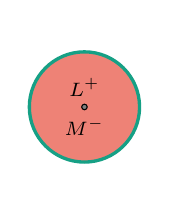
\begin{tikzpicture}
            % Frame to ensure alignment:
            \draw[opacity=0]                                           ( 0.00, -1.00) --     (0.00, 1.00);
            \filldraw[greensea,    fill=alizarin!70,  very thick]( 0.00,  0.00) circle (0.70)
                 node[color=black,       anchor=south] {$\scriptstyle L^+$}
                 node[color=black,       anchor=north] {$\scriptstyle M^-$};
            \filldraw[color=black,       fill=gray]                    ( 0.00,  0.00) circle (1pt);
        \end{tikzpicture}
        \caption{Symmetric \\ balanced \\ single-opponent \\ receptive field}
    \end{subfigure}%
    \begin{subfigure}{0.3\textwidth}
        \centering
        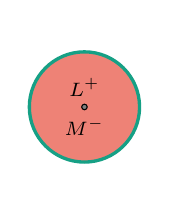
\begin{tikzpicture}
            % Frame to ensure alignment:
            \draw[opacity=0]                                           ( 0.00, -1.00) --     (0.00, 1.00);
            \filldraw[greensea,    fill=alizarin!70,  very thick]( 0.00,  0.00) circle (0.70)
                 node[color=black,       anchor=south] {$\scriptstyle L^+$}
                 node[color=black,       anchor=north] {$\scriptstyle M^-$};
            \filldraw[color=black,       fill=gray]                    ( 0.00,  0.00) circle (1pt);
        \end{tikzpicture}
        \caption{Symmetric \\ imbalanced \\ single-opponent \\ receptive field}
    \end{subfigure}%
    \begin{subfigure}{0.3\textwidth}
        \centering
        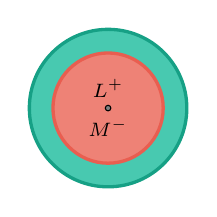
\begin{tikzpicture}
            \filldraw[greensea,    fill=turquoise!80, very thick]( 0.00,  0.00) circle (1.00);
            \filldraw[color=alizarin!90, fill=alizarin!70,  very thick]( 0.00,  0.00) circle (0.70)
                 node[color=black,       anchor=south] {$\scriptstyle L^+$}
                 node[color=black,       anchor=north] {$\scriptstyle M^-$};
            \filldraw[color=black,       fill=gray]                    ( 0.00,  0.00) circle (1pt);
        \end{tikzpicture}
        \caption{Classic \\ center/surround \\ single-opponent \\ receptive field}
    \end{subfigure}%
    \caption{Examples of various possible single-opponent receptive field configurations, many others could be designed. All function to describe color properties of surfaces, though their response patterns to similar stimuli vary slightly.}
\end{figure}


% FIGURE: Double-opponent receptive field schematics
\begin{figure}[h] \label{fig:do-rf-schematic}
    \centering
    \captionsetup{justification=centering}
    % 3 SUBFIGURES: Cross sections of double-opponent receptive fields
    \begin{subfigure}{0.3\textwidth}
        \centering
        \resizebox{\textwidth}{!}{%
        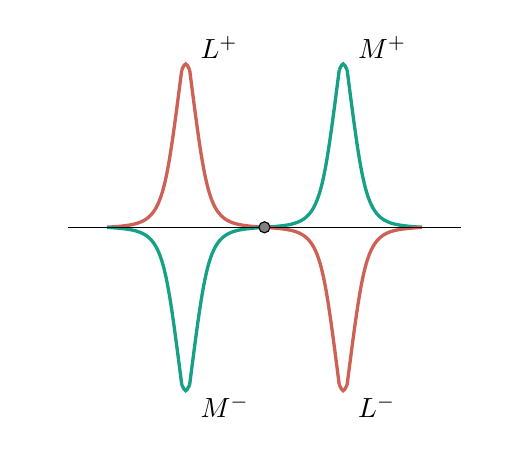
\begin{tikzpicture}
            % ON Center
            \draw[pomegranate!80, very thick] (-2.00, 0.00) .. controls (-1.30, 0.05) .. (-1.05, 2.00);
            \draw[pomegranate!80, very thick] (-1.05, 2.00) .. controls (-1.00, 2.10) .. (-0.95, 2.00);
            \draw[pomegranate!80, very thick] ( 0.00, 0.00) .. controls (-0.70, 0.05) .. (-0.95, 2.00)
                 node[color=black, anchor=south west] {$L^+$};
            % OFF Surround
            \draw[greensea,       very thick] (-2.00, 0.00) .. controls (-1.30,-0.05) .. (-1.05,-2.00);
            \draw[greensea,       very thick] (-1.05,-2.00) .. controls (-1.00,-2.10) .. (-0.95,-2.00);
            \draw[greensea,       very thick] ( 0.00, 0.00) .. controls (-0.70,-0.05) .. (-0.95,-2.00)
                 node[color=black, anchor=north west] {$M^-$};
            % ON Center
            \draw[greensea,       very thick] ( 0.00, 0.00) .. controls ( 0.70, 0.05) .. ( 0.95, 2.00);
            \draw[greensea,       very thick] ( 1.05, 2.00) .. controls ( 1.00, 2.10) .. ( 0.95, 2.00);
            \draw[greensea,       very thick] ( 2.00, 0.00) .. controls ( 1.30, 0.05) .. ( 1.05, 2.00)
                 node[color=black, anchor=south west] {$M^+$};
            % OFF Surround
            \draw[pomegranate!80, very thick] ( 0.00, 0.00) .. controls ( 0.70,-0.05) .. ( 0.95,-2.00);
            \draw[pomegranate!80, very thick] ( 1.05,-2.00) .. controls ( 1.00,-2.10) .. ( 0.95,-2.00);
            \draw[pomegranate!80, very thick] ( 2.00, 0.00) .. controls ( 1.30,-0.05) .. ( 1.05,-2.00)
                 node[color=black, anchor=north west] {$L^-$};
            % Reference line & point
            \draw                                                             (-2.50, 0.00) -- ( 2.50, 0.00);
            \filldraw[color=black, fill=gray]                                 ( 0.00, 0.00) circle (2pt);
            % Frame to ensure alignment:
            \draw[opacity=0]                                                  (-3.00, 2.50) rectangle (3.00, -2.50);
        \end{tikzpicture}}
    \end{subfigure}
    \begin{subfigure}{0.3\textwidth}
        \resizebox{\textwidth}{!}{%
        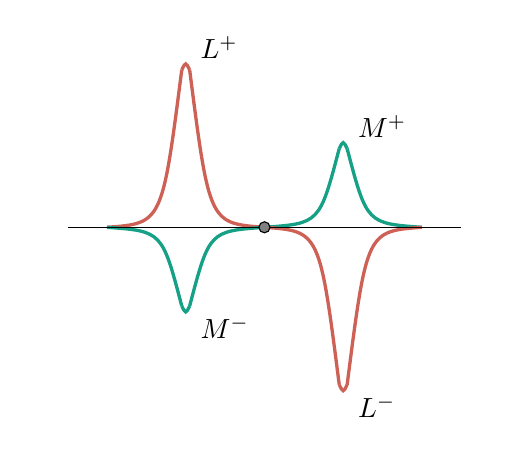
\begin{tikzpicture}
            % ON Center
            \draw[pomegranate!80, very thick] (-2.00, 0.00) .. controls (-1.30, 0.05) .. (-1.05, 2.00);
            \draw[pomegranate!80, very thick] (-1.05, 2.00) .. controls (-1.00, 2.10) .. (-0.95, 2.00);
            \draw[pomegranate!80, very thick] ( 0.00, 0.00) .. controls (-0.70, 0.05) .. (-0.95, 2.00)
                 node[color=black, anchor=south west] {$L^+$};
            % OFF Surround
            \draw[greensea,       very thick] (-2.00, 0.00) .. controls (-1.30,-0.05) .. (-1.05,-1.00);
            \draw[greensea,       very thick] (-1.05,-1.00) .. controls (-1.00,-1.10) .. (-0.95,-1.00);
            \draw[greensea,       very thick] ( 0.00, 0.00) .. controls (-0.70,-0.05) .. (-0.95,-1.00)
                 node[color=black, anchor=north west] {$M^-$};
            % ON Center
            \draw[greensea,       very thick] ( 0.00, 0.00) .. controls ( 0.70, 0.05) .. ( 0.95, 1.00);
            \draw[greensea,       very thick] ( 1.05, 1.00) .. controls ( 1.00, 1.10) .. ( 0.95, 1.00);
            \draw[greensea,       very thick] ( 2.00, 0.00) .. controls ( 1.30, 0.05) .. ( 1.05, 1.00)
                 node[color=black, anchor=south west] {$M^+$};
            % OFF Surround
            \draw[pomegranate!80, very thick] ( 0.00, 0.00) .. controls ( 0.70,-0.05) .. ( 0.95,-2.00);
            \draw[pomegranate!80, very thick] ( 1.05,-2.00) .. controls ( 1.00,-2.10) .. ( 0.95,-2.00);
            \draw[pomegranate!80, very thick] ( 2.00, 0.00) .. controls ( 1.30,-0.05) .. ( 1.05,-2.00)
                 node[color=black, anchor=north west] {$L^-$};
            % Reference line & point
            \draw                                                             (-2.50, 0.00) -- ( 2.50, 0.00);
            \filldraw[color=black, fill=gray]                                 ( 0.00, 0.00) circle (2pt);
            % Frame to ensure alignment:
            \draw[opacity=0]                                                  (-3.00, 2.50) rectangle (3.00, -2.50);
        \end{tikzpicture}}
    \end{subfigure}
    \begin{subfigure}{0.3\textwidth}
        \resizebox{\textwidth}{!}{%
        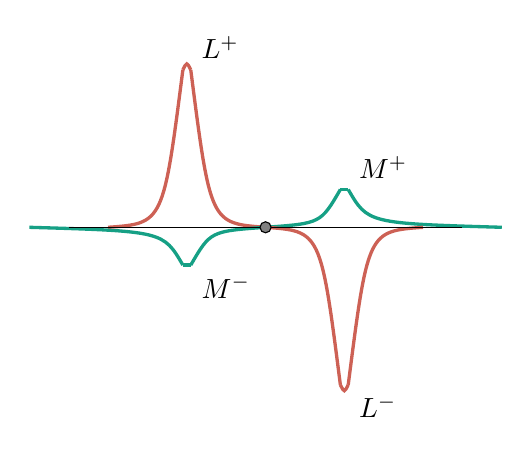
\begin{tikzpicture}
            % ON Center
            \draw[pomegranate!80, very thick] (-2.00, 0.00) .. controls (-1.30, 0.05) .. (-1.05, 2.00);
            \draw[pomegranate!80, very thick] (-1.05, 2.00) .. controls (-1.00, 2.10) .. (-0.95, 2.00);
            \draw[pomegranate!80, very thick] ( 0.00, 0.00) .. controls (-0.70, 0.05) .. (-0.95, 2.00)
                 node[color=black, anchor=south west] {$L^+$};
            % OFF Surround
            \draw[greensea,       very thick] (-3.00, 0.00) .. controls (-1.30,-0.05) .. (-1.05,-0.48);
            \draw[greensea,       very thick] (-1.05,-0.48) .. controls (-1.00,-0.49) .. (-0.95,-0.48);
            \draw[greensea,       very thick] ( 0.00, 0.00) .. controls (-0.70,-0.05) .. (-0.95,-0.48)
                 node[color=black, anchor=north west] {$M^-$};
            % ON Center
            \draw[greensea,       very thick] ( 0.00, 0.00) .. controls ( 0.70, 0.05) .. ( 0.95, 0.48);
            \draw[greensea,       very thick] ( 1.05, 0.48) .. controls ( 1.00, 0.49) .. ( 0.95, 0.48);
            \draw[greensea,       very thick] ( 3.00, 0.00) .. controls ( 1.30, 0.05) .. ( 1.05, 0.48)
                 node[color=black, anchor=south west] {$M^+$};
            % OFF Surround
            \draw[pomegranate!80, very thick] ( 0.00, 0.00) .. controls ( 0.70,-0.05) .. ( 0.95,-2.00);
            \draw[pomegranate!80, very thick] ( 1.05,-2.00) .. controls ( 1.00,-2.10) .. ( 0.95,-2.00);
            \draw[pomegranate!80, very thick] ( 2.00, 0.00) .. controls ( 1.30,-0.05) .. ( 1.05,-2.00)
                 node[color=black, anchor=north west] {$L^-$};
            % Reference line & point
            \draw                                                             (-2.50, 0.00) -- ( 2.50, 0.00);
            \filldraw[color=black, fill=gray]                                 ( 0.00, 0.00) circle (2pt);
            % Frame to ensure alignment:
            \draw[opacity=0]                                                  (-3.00, 2.50) rectangle (3.00, -2.50);
        \end{tikzpicture}}
    \end{subfigure}%
    \par \bigskip
    % 3 SUBFIGURES: Top-down view of double-opponent receptive fields
    \begin{subfigure}{0.3\textwidth}
        \centering
        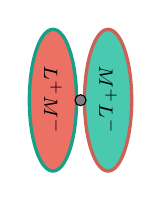
\begin{tikzpicture}
            \filldraw[pomegranate!80,       fill=turquoise!80, very thick]( 0.35, 0.00) ellipse   (0.30 and 0.90)
                 node[color=black, anchor=center, rotate=-90] {$\scriptstyle M^+L^-$};
            \filldraw[greensea, fill=alizarin!80,  very thick](-0.35, 0.00) ellipse   (0.30 and 0.90)
                 node[color=black, anchor=center, rotate=-90] {$\scriptstyle L^+M^-$};
            \filldraw[color=black,          fill=gray]                    ( 0.00, 0.00) circle    (2pt);
        \end{tikzpicture}
        \caption{Symmetric \\ balanced \\ double-opponent \\ receptive field}
    \end{subfigure}%
    \begin{subfigure}{0.3\textwidth}
        \centering
        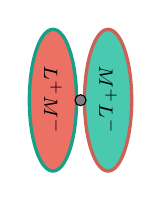
\begin{tikzpicture}
            \filldraw[pomegranate!80,       fill=turquoise!80, very thick]( 0.35, 0.00) ellipse   (0.30 and 0.90)
                 node[color=black, anchor=center, rotate=-90] {$\scriptstyle M^+L^-$};
            \filldraw[greensea, fill=alizarin!80,  very thick](-0.35, 0.00) ellipse   (0.30 and 0.90)
                 node[color=black, anchor=center, rotate=-90] {$\scriptstyle L^+M^-$};
            \filldraw[color=black,          fill=gray]                    ( 0.00, 0.00) circle    (2pt);
        \end{tikzpicture}
        \caption{Symmetric \\ imbalanced \\ double-opponent \\ receptive field}
    \end{subfigure}%
    \begin{subfigure}{0.3\textwidth}
        \centering
        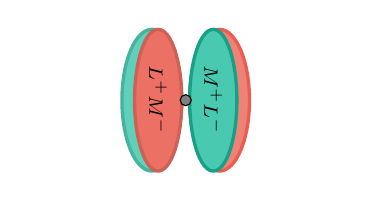
\begin{tikzpicture}
            % Frame to ensure alignment:
            \draw[opacity=0]                                              (-2.00, 0.00) --        (2.00, 0.00);
            \filldraw[color=alizarin!90,    fill=alizarin!70,  very thick]( 0.43, 0.00) ellipse   (0.38 and 0.90);
            \filldraw[greensea!80,    fill=turquoise!70, very thick](-0.43, 0.00) ellipse   (0.38 and 0.90);
            \filldraw[greensea,       fill=turquoise!80, very thick]( 0.35, 0.00) ellipse   (0.30 and 0.90)
                 node[color=black, anchor=center, rotate=-90] {$\scriptstyle M^+L^-$};
            \filldraw[pomegranate!80, fill=alizarin!80,  very thick](-0.35, 0.00) ellipse   (0.30 and 0.90)
                 node[color=black, anchor=center, rotate=-90] {$\scriptstyle L^+M^-$};
            \filldraw[color=black,          fill=gray]                    ( 0.00, 0.00) circle    (2pt);
        \end{tikzpicture}
        \caption{Center/ \\ surround \\ double-opponent \\ receptive field}
    \end{subfigure}%
    \caption{Examples of various possible double-opponent receptive field configurations, many others could be designed. All function to describe color properties of borders, though their response patterns to similar stimuli vary slightly.}
\end{figure}


% FIGURE: Oriented double-opponent receptive fields
\begin{figure}[h] \label{fig:dos}
    \centering
    \captionsetup{justification=centering}
    % Horizontal Double-Opponent Receptive Fields
    \begin{subfigure}{0.5\textwidth}
        \centering
        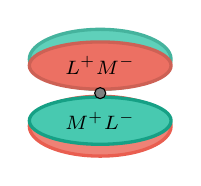
\begin{tikzpicture}
            \filldraw[greensea!80,    fill=turquoise!70, very thick]( 0.00, 1.43) ellipse   (0.90 and 0.38);
            \filldraw[color=alizarin!90,    fill=alizarin!70,  very thick]( 0.00, 0.58) ellipse   (0.90 and 0.38);
            \filldraw[pomegranate!80, fill=alizarin!80,  very thick]( 0.00, 1.35) ellipse   (0.90 and 0.30)
                 node[color=black, anchor=center] {$\scriptstyle L^+M^-$};
            \filldraw[greensea,       fill=turquoise!80, very thick]( 0.00, 0.65) ellipse   (0.90 and 0.30)
                 node[color=black, anchor=center] {$\scriptstyle M^+L^-$};
            \filldraw[color=black,          fill=gray]                    ( 0.00, 1.00) circle    (2pt);
        \end{tikzpicture}
        \caption{Vertical $R$ vs. $G$ double-opponent \\ cell receptive fields.}
    \end{subfigure}%
    \begin{subfigure}{0.5\textwidth}
        \centering
        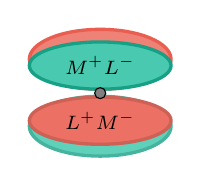
\begin{tikzpicture}
            \filldraw[color=alizarin!90,    fill=alizarin!70,  very thick]( 0.00, 1.43) ellipse   (0.90 and 0.38);
            \filldraw[greensea!80,    fill=turquoise!70, very thick]( 0.00, 0.58) ellipse   (0.90 and 0.38);
            \filldraw[greensea,       fill=turquoise!80, very thick]( 0.00, 1.35) ellipse   (0.90 and 0.30)
                 node[color=black, anchor=center] {$\scriptstyle M^+L^-$};
            \filldraw[pomegranate!80, fill=alizarin!80,  very thick]( 0.00, 0.65) ellipse   (0.90 and 0.30)
                 node[color=black, anchor=center] {$\scriptstyle L^+M^-$};
            \filldraw[color=black,          fill=gray]                    ( 0.00, 1.00) circle    (2pt);
        \end{tikzpicture}
        \caption{Vertical $G$ vs. $R$ double-opponent \\ cell receptive fields.}
    \end{subfigure}%
    \par \bigskip
    % Diagonal Double-Opponent Receptive Fields #1
    \begin{subfigure}{0.5\textwidth}
        \centering
        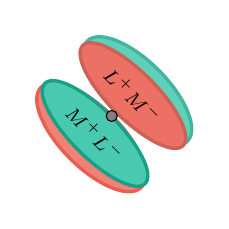
\begin{tikzpicture}
            \filldraw[greensea!80,    fill=turquoise!70, very thick, rotate=45]( 1.16, 0.70) ellipse   (0.38 and 0.90);
            \filldraw[color=alizarin!90,    fill=alizarin!70,  very thick, rotate=45]( 0.33, 0.70) ellipse   (0.38 and 0.90);
            \filldraw[pomegranate!80, fill=alizarin!80,  very thick, rotate=45]( 1.08, 0.70) ellipse   (0.30 and 0.90)
                 node[color=black, anchor=center, rotate=-45] {$\scriptstyle L^+M^-$};
            \filldraw[greensea,       fill=turquoise!80, very thick, rotate=45]( 0.40, 0.70) ellipse   (0.30 and 0.90)
                 node[color=black, anchor=center, rotate=-45] {$\scriptstyle M^+L^-$};
            \filldraw[color=black,          fill=gray]                    ( 0.00, 1.00) circle    (2pt);
        \end{tikzpicture}
        \caption{Diagonal $R$ vs. $G$ double-opponent \\ cell receptive fields.}
    \end{subfigure}%
    \begin{subfigure}{0.5\textwidth}
        \centering
        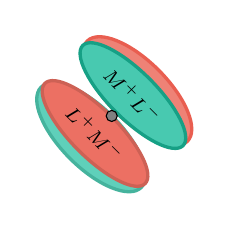
\begin{tikzpicture}
            \filldraw[color=alizarin!90,    fill=alizarin!70,  very thick, rotate=45]( 1.16, 0.70) ellipse   (0.38 and 0.90);
            \filldraw[greensea!80,    fill=turquoise!70, very thick, rotate=45]( 0.33, 0.70) ellipse   (0.38 and 0.90);
            \filldraw[greensea,       fill=turquoise!80, very thick, rotate=45]( 1.08, 0.70) ellipse   (0.30 and 0.90)
                 node[color=black, anchor=center, rotate=-45] {$\scriptstyle M^+L^-$};
            \filldraw[pomegranate!80, fill=alizarin!80,  very thick, rotate=45]( 0.40, 0.70) ellipse   (0.30 and 0.90)
                 node[color=black, anchor=center, rotate=-45] {$\scriptstyle L^+M^-$};
            \filldraw[color=black,          fill=gray]                    ( 0.00, 1.00) circle    (2pt);
        \end{tikzpicture}
        \caption{Diagonal $G$ vs. $R$ double-opponent \\ cell receptive fields.}
    \end{subfigure}%
    \par \bigskip
    % Vertical Double-Opponent Receptive Fields
    \begin{subfigure}{0.5\textwidth}
        \centering
        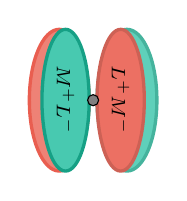
\begin{tikzpicture}
            \filldraw[greensea!80,    fill=turquoise!70, very thick]( 0.43, 1.00) ellipse   (0.38 and 0.90);
            \filldraw[color=alizarin!90,    fill=alizarin!70,  very thick](-0.43, 1.00) ellipse   (0.38 and 0.90);
            \filldraw[pomegranate!80, fill=alizarin!80,  very thick]( 0.35, 1.00) ellipse   (0.30 and 0.90)
                 node[color=black, anchor=center, rotate=-90] {$\scriptstyle L^+M^-$};
            \filldraw[greensea,       fill=turquoise!80, very thick](-0.35, 1.00) ellipse   (0.30 and 0.90)
                 node[color=black, anchor=center, rotate=-90] {$\scriptstyle M^+L^-$};
            \filldraw[color=black,          fill=gray]                    ( 0.00, 1.00) circle    (2pt);
        \end{tikzpicture}
        \caption{Horizontal $R$ vs. $G$ double-opponent \\ cell receptive fields.}
    \end{subfigure}%
    \begin{subfigure}{0.5\textwidth}
        \centering
        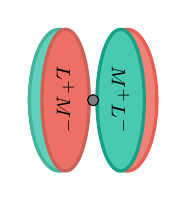
\begin{tikzpicture}
            \filldraw[color=alizarin!90,    fill=alizarin!70,  very thick]( 0.43, 1.00) ellipse   (0.38 and 0.90);
            \filldraw[greensea!80,    fill=turquoise!70, very thick](-0.43, 1.00) ellipse   (0.38 and 0.90);
            \filldraw[greensea,       fill=turquoise!80, very thick]( 0.35, 1.00) ellipse   (0.30 and 0.90)
                 node[color=black, anchor=center, rotate=-90] {$\scriptstyle M^+L^-$};
            \filldraw[pomegranate!80, fill=alizarin!80,  very thick](-0.35, 1.00) ellipse   (0.30 and 0.90)
                 node[color=black, anchor=center, rotate=-90] {$\scriptstyle L^+M^-$};
            \filldraw[color=black,          fill=gray]                    ( 0.00, 1.00) circle    (2pt);
        \end{tikzpicture}
        \caption{Horizontal $G$ vs. $R$ double-opponent \\ cell receptive fields.}
    \end{subfigure}%
    \par \bigskip
    % Diagonal Double-Opponent Receptive Fields #2
    \begin{subfigure}{0.5\textwidth}
        \centering
        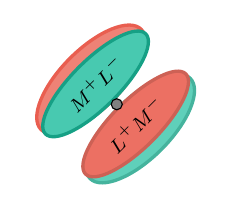
\begin{tikzpicture}
            \filldraw[color=alizarin!90,    fill=alizarin!70, very thick, rotate=45]( 0.70, 1.16) ellipse   (0.90 and 0.38);
            \filldraw[greensea!80,    fill=turquoise!70,  very thick, rotate=45]( 0.70, 0.28) ellipse   (0.90 and 0.38);
            \filldraw[greensea,       fill=turquoise!80,  very thick, rotate=45]( 0.70, 1.08) ellipse   (0.90 and 0.30)
                 node[color=black, anchor=center, rotate=45] {$\scriptstyle M^+L^-$};
            \filldraw[pomegranate!80, fill=alizarin!80, very thick, rotate=45]( 0.70, 0.36) ellipse   (0.90 and 0.30)
                 node[color=black, anchor=center, rotate=45] {$\scriptstyle L^+M^-$};
            \filldraw[color=black,          fill=gray]                    ( 0.00, 1.00) circle    (2pt);
        \end{tikzpicture}
        \caption{Diagonal $R$ vs. $G$ double-opponent \\ cell receptive fields.}
    \end{subfigure}%
    \begin{subfigure}{0.5\textwidth}
        \centering
        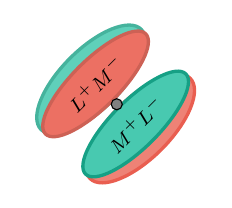
\begin{tikzpicture}
            \filldraw[greensea!80,    fill=turquoise!70, very thick, rotate=45]( 0.70, 1.16) ellipse   (0.90 and 0.38);
            \filldraw[color=alizarin!90,    fill=alizarin!70,  very thick, rotate=45]( 0.70, 0.28) ellipse   (0.90 and 0.38);
            \filldraw[pomegranate!80, fill=alizarin!80,  very thick, rotate=45]( 0.70, 1.08) ellipse   (0.90 and 0.30)
                 node[color=black, anchor=center, rotate=45] {$\scriptstyle L^+M^-$};
            \filldraw[greensea,       fill=turquoise!80, very thick, rotate=45]( 0.70, 0.36) ellipse   (0.90 and 0.30)
                 node[color=black, anchor=center, rotate=45] {$\scriptstyle M^+L^-$};
            \filldraw[color=black,          fill=gray]                    ( 0.00, 1.00) circle    (2pt);
        \end{tikzpicture}
        \caption{Diagonal $R$ vs. $G$ double-opponent \\ cell receptive fields.}
    \end{subfigure}%
    \caption{Schematic of orientation selectivity in double-opponent receptive field configurations. Any single double-opponent neuron only has one receptive field hard wired into it. By having collections of neurons, each selective to a different orientation at the same retinotopic location, we obtain a degree of rotation invariance.}
\end{figure}


% FIGURE: horizontal red/green double-opponent cell on horizontal red/green border
\begin{figure}[h] \label{fig:do-orient-h}
    \centering
    \begin{subfigure}{0.2\textwidth}
        \centering
        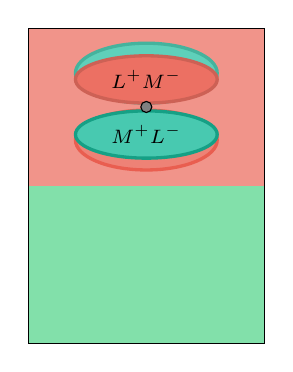
\begin{tikzpicture}
            \fill[alizarin!60]                                            (-1.50, 2.00) rectangle (1.50, 0.00);
            \fill[emerald!60]                                             (-1.50,-2.00) rectangle (1.50, 0.00);
            \filldraw[greensea!80,    fill=turquoise!70, very thick]( 0.00, 1.43) ellipse   (0.90 and 0.38);
            \filldraw[color=alizarin!90,    fill=alizarin!70,  very thick]( 0.00, 0.58) ellipse   (0.90 and 0.38);
            \filldraw[pomegranate!80, fill=alizarin!80,  very thick]( 0.00, 1.35) ellipse   (0.90 and 0.30)
                 node[color=black, anchor=center] {$\scriptstyle L^+M^-$};
            \filldraw[greensea,       fill=turquoise!80, very thick]( 0.00, 0.65) ellipse   (0.90 and 0.30)
                 node[color=black, anchor=center] {$\scriptstyle M^+L^-$};
            \filldraw[color=black,          fill=gray]                    ( 0.00, 1.00) circle    (2pt);
            \draw (current bounding box.north east) rectangle (current bounding box.south west);
        \end{tikzpicture}
        \caption{Minor Response}
    \end{subfigure}%
    \begin{subfigure}{0.2\textwidth}
        \centering
        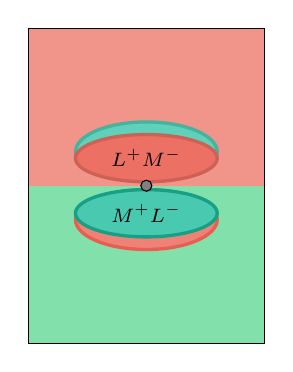
\begin{tikzpicture}
            \fill[alizarin!60]                                            (-1.50, 2.00) rectangle (1.50, 0.00);
            \fill[emerald!60]                                             (-1.50,-2.00) rectangle (1.50, 0.00);
            \filldraw[greensea!80,    fill=turquoise!70, very thick]( 0.00, 0.43) ellipse   (0.90 and 0.38);
            \filldraw[color=alizarin!90,    fill=alizarin!70,  very thick]( 0.00,-0.43) ellipse   (0.90 and 0.38);
            \filldraw[pomegranate!80, fill=alizarin!80,  very thick]( 0.00, 0.35) ellipse   (0.90 and 0.30)
                 node[color=black, anchor=center] {$\scriptstyle L^+M^-$};
            \filldraw[greensea,       fill=turquoise!80, very thick]( 0.00,-0.35) ellipse   (0.90 and 0.30)
                 node[color=black, anchor=center] {$\scriptstyle M^+L^-$};
            \filldraw[color=black,          fill=gray]                    ( 0.00, 0.00) circle    (2pt);
        \draw (current bounding box.north east) rectangle (current bounding box.south west);
        \end{tikzpicture}
        \caption{Maximum Response}
    \end{subfigure}%
    \begin{subfigure}{0.2\textwidth}
        \centering
        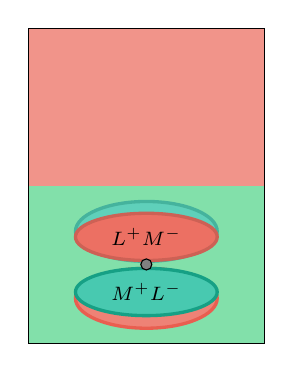
\begin{tikzpicture}
            \fill[alizarin!60]                                            (-1.50, 2.00) rectangle (1.50, 0.00);
            \fill[emerald!60]                                             (-1.50,-2.00) rectangle (1.50, 0.00);
            \filldraw[greensea!80,    fill=turquoise!70, very thick]( 0.00,-0.58) ellipse   (0.90 and 0.38);
            \filldraw[color=alizarin!90,    fill=alizarin!70,  very thick]( 0.00,-1.43) ellipse   (0.90 and 0.38);
            \filldraw[pomegranate!80, fill=alizarin!80,  very thick]( 0.00,-0.65) ellipse   (0.90 and 0.30)
                 node[color=black, anchor=center] {$\scriptstyle L^+M^-$};
            \filldraw[greensea,       fill=turquoise!80, very thick]( 0.00,-1.35) ellipse   (0.90 and 0.30)
                 node[color=black, anchor=center] {$\scriptstyle M^+L^-$};
            \filldraw[color=black,          fill=gray]                    ( 0.00,-1.00) circle    (2pt);
        \draw (current bounding box.north east) rectangle (current bounding box.south west);
        \end{tikzpicture}
        \caption{Minor Response}
    \end{subfigure}%
    \par \bigskip
    \begin{subfigure}{0.2\textwidth}
        \centering
        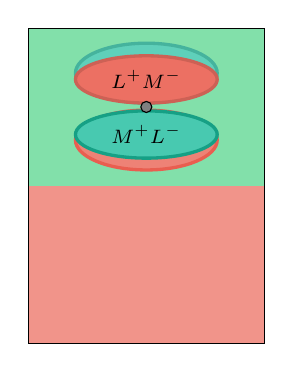
\begin{tikzpicture}
            \fill[emerald!60]                                             (-1.50, 2.00) rectangle (1.50, 0.00);
            \fill[alizarin!60]                                            (-1.50,-2.00) rectangle (1.50, 0.00);
            \filldraw[greensea!80,    fill=turquoise!70, very thick]( 0.00, 1.43) ellipse   (0.90 and 0.38);
            \filldraw[color=alizarin!90,    fill=alizarin!70,  very thick]( 0.00, 0.58) ellipse   (0.90 and 0.38);
            \filldraw[pomegranate!80, fill=alizarin!80,  very thick]( 0.00, 1.35) ellipse   (0.90 and 0.30)
                 node[color=black, anchor=center] {$\scriptstyle L^+M^-$};
            \filldraw[greensea,       fill=turquoise!80, very thick]( 0.00, 0.65) ellipse   (0.90 and 0.30)
                 node[color=black, anchor=center] {$\scriptstyle M^+L^-$};
            \filldraw[color=black,          fill=gray]                    ( 0.00, 1.00) circle    (2pt);
            \draw (current bounding box.north east) rectangle (current bounding box.south west);
        \end{tikzpicture}
        \caption{Minor Response}
    \end{subfigure}%
    \begin{subfigure}{0.2\textwidth}
        \centering
        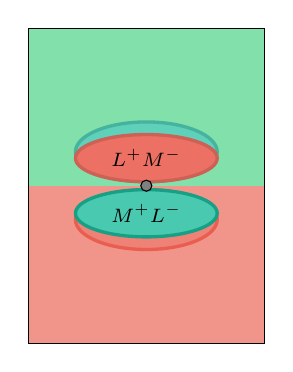
\begin{tikzpicture}
            \fill[emerald!60]                                             (-1.50, 2.00) rectangle (1.50, 0.00);
            \fill[alizarin!60]                                            (-1.50,-2.00) rectangle (1.50, 0.00);
            \filldraw[greensea!80,    fill=turquoise!70, very thick]( 0.00, 0.43) ellipse   (0.90 and 0.38);
            \filldraw[color=alizarin!90,    fill=alizarin!70,  very thick]( 0.00,-0.43) ellipse   (0.90 and 0.38);
            \filldraw[pomegranate!80, fill=alizarin!80,  very thick]( 0.00, 0.35) ellipse   (0.90 and 0.30)
                 node[color=black, anchor=center] {$\scriptstyle L^+M^-$};
            \filldraw[greensea,       fill=turquoise!80, very thick]( 0.00,-0.35) ellipse   (0.90 and 0.30)
                 node[color=black, anchor=center] {$\scriptstyle M^+L^-$};
            \filldraw[color=black,          fill=gray]                    ( 0.00, 0.00) circle    (2pt);
        \draw (current bounding box.north east) rectangle (current bounding box.south west);
        \end{tikzpicture}
        \caption{No Response}
    \end{subfigure}%
    \begin{subfigure}{0.2\textwidth}
        \centering
        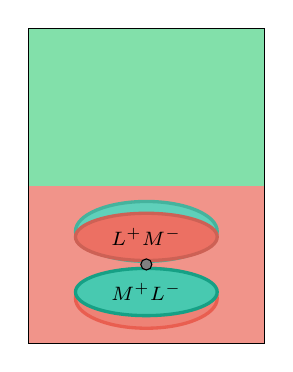
\begin{tikzpicture}
            \fill[emerald!60]                                             (-1.50, 2.00) rectangle (1.50, 0.00);
            \fill[alizarin!60]                                            (-1.50,-2.00) rectangle (1.50, 0.00);
            \filldraw[greensea!80,    fill=turquoise!70, very thick]( 0.00,-0.58) ellipse   (0.90 and 0.38);
            \filldraw[color=alizarin!90,    fill=alizarin!70,  very thick]( 0.00,-1.43) ellipse   (0.90 and 0.38);
            \filldraw[pomegranate!80, fill=alizarin!80,  very thick]( 0.00,-0.65) ellipse   (0.90 and 0.30)
                 node[color=black, anchor=center] {$\scriptstyle L^+M^-$};
            \filldraw[greensea,       fill=turquoise!80, very thick]( 0.00,-1.35) ellipse   (0.90 and 0.30)
                 node[color=black, anchor=center] {$\scriptstyle M^+L^-$};
            \filldraw[color=black,          fill=gray]                    ( 0.00,-1.00) circle    (2pt);
        \draw (current bounding box.north east) rectangle (current bounding box.south west);
        \end{tikzpicture}
        \caption{Minor Response}
    \end{subfigure}
    \caption{A double-opponent cell selective to horizontally oriented borders with red above and green below; only responsive to that particular stimulus. In Figure (b), the neuron is presented with its ideal stimulus: its $L^+$ and $M^+$ receptive fields are fully activated while its $L^-$ and $M^-$ receptive fields are completely unactivated. Figure (e) presents the neuron with the exact opposite stimulus, neither its $L^+$ nor $M^+$ receptive fields are activate at all, and both its $L^-$ and $M^-$ receptive fields are fully activated, ensuring no response possible from the cell. While its $L^+$ receptive field might be strongly stimulated in (a) and (f), it's $L^-$ receptive field cancels it out. Similarly, in (c) and (d) its $M^+$ receptive field is stimulated but cancelled out by activity in its $M^-$ receptive field.}
\end{figure}


% FIGURE: vertical red/green double-opponent cell on horizontal red/green border
\begin{figure}[h] \label{fig:do-orient-v}
    \centering
    \begin{subfigure}{0.2\textwidth}
        \centering
        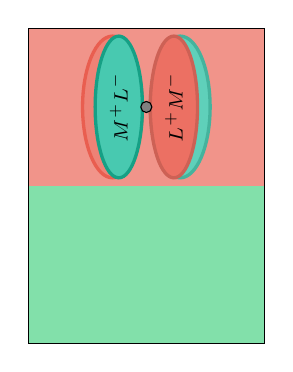
\begin{tikzpicture}
            \fill[alizarin!60]                                            (-1.50, 2.00) rectangle (1.50, 0.00);
            \fill[emerald!60]                                             (-1.50,-2.00) rectangle (1.50, 0.00);
            \filldraw[greensea!80,    fill=turquoise!70, very thick]( 0.43, 1.00) ellipse   (0.38 and 0.90);
            \filldraw[color=alizarin!90,    fill=alizarin!70,  very thick](-0.43, 1.00) ellipse   (0.38 and 0.90);
            \filldraw[pomegranate!80, fill=alizarin!80,  very thick]( 0.35, 1.00) ellipse   (0.30 and 0.90)
                 node[color=black, anchor=center, rotate=90] {$\scriptstyle L^+M^-$};
            \filldraw[greensea,       fill=turquoise!80, very thick](-0.35, 1.00) ellipse   (0.30 and 0.90)
                 node[color=black, anchor=center, rotate=90] {$\scriptstyle M^+L^-$};
            \filldraw[color=black,          fill=gray]                    ( 0.00, 1.00) circle    (2pt);
            \draw (current bounding box.north east) rectangle (current bounding box.south west);
        \end{tikzpicture}
        \caption{Minor Response}
    \end{subfigure}%
    \begin{subfigure}{0.2\textwidth}
        \centering
            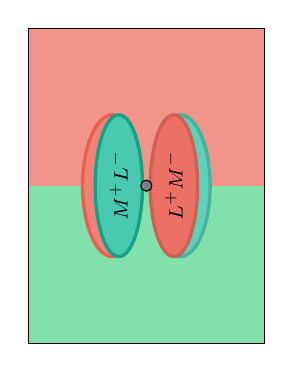
\begin{tikzpicture}
            \fill[alizarin!60]                                            (-1.50, 2.00) rectangle (1.50, 0.00);
            \fill[emerald!60]                                             (-1.50,-2.00) rectangle (1.50, 0.00);
            \filldraw[greensea!80,    fill=turquoise!70, very thick]( 0.43, 0.00) ellipse   (0.38 and 0.90);
            \filldraw[color=alizarin!90,    fill=alizarin!70,  very thick](-0.43, 0.00) ellipse   (0.38 and 0.90);
            \filldraw[pomegranate!80, fill=alizarin!80,  very thick]( 0.35, 0.00) ellipse   (0.30 and 0.90)
                 node[color=black, anchor=center, rotate=90] {$\scriptstyle L^+M^-$};
            \filldraw[greensea,       fill=turquoise!80, very thick](-0.35, 0.00) ellipse   (0.30 and 0.90)
                 node[color=black, anchor=center, rotate=90] {$\scriptstyle M^+L^-$};
            \filldraw[color=black,          fill=gray]                    ( 0.00, 0.00) circle    (2pt);
            \draw (current bounding box.north east) rectangle (current bounding box.south west);
            \end{tikzpicture}
        \caption{Minimal Response}
    \end{subfigure}%
    \begin{subfigure}{0.2\textwidth}
        \centering
            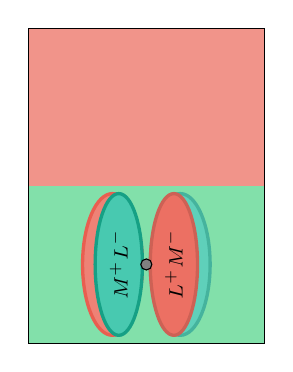
\begin{tikzpicture}
            \fill[alizarin!60]                                            (-1.50, 2.00) rectangle (1.50, 0.00);
            \fill[emerald!60]                                             (-1.50,-2.00) rectangle (1.50, 0.00);
            \filldraw[greensea!80,    fill=turquoise!70, very thick]( 0.43,-1.00) ellipse   (0.38 and 0.90);
            \filldraw[color=alizarin!90,    fill=alizarin!70,  very thick](-0.43,-1.00) ellipse   (0.38 and 0.90);
            \filldraw[pomegranate!80, fill=alizarin!80,  very thick]( 0.35,-1.00) ellipse   (0.30 and 0.90)
                 node[color=black, anchor=center, rotate=90] {$\scriptstyle L^+M^-$};
            \filldraw[greensea,       fill=turquoise!80, very thick](-0.35,-1.00) ellipse   (0.30 and 0.90)
                 node[color=black, anchor=center, rotate=90] {$\scriptstyle M^+L^-$};
            \filldraw[color=black,          fill=gray]                    ( 0.00,-1.00) circle    (2pt);
            \draw (current bounding box.north east) rectangle (current bounding box.south west);
            \end{tikzpicture}
        \caption{Minor Response}
    \end{subfigure}%
    \par \bigskip
    \begin{subfigure}{0.2\textwidth}
        \centering
        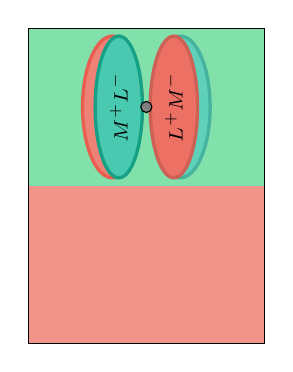
\begin{tikzpicture}
            \fill[emerald!60]                                             (-1.50, 2.00) rectangle (1.50, 0.00);
            \fill[alizarin!60]                                            (-1.50,-2.00) rectangle (1.50, 0.00);
            \filldraw[greensea!80,    fill=turquoise!70, very thick]( 0.43, 1.00) ellipse   (0.38 and 0.90);
            \filldraw[color=alizarin!90,    fill=alizarin!70,  very thick](-0.43, 1.00) ellipse   (0.38 and 0.90);
            \filldraw[pomegranate!80, fill=alizarin!80,  very thick]( 0.35, 1.00) ellipse   (0.30 and 0.90)
                 node[color=black, anchor=center, rotate=90] {$\scriptstyle L^+M^-$};
            \filldraw[greensea,       fill=turquoise!80, very thick](-0.35, 1.00) ellipse   (0.30 and 0.90)
                 node[color=black, anchor=center, rotate=90] {$\scriptstyle M^+L^-$};
            \filldraw[color=black,          fill=gray]                    ( 0.00, 1.00) circle    (2pt);
            \draw (current bounding box.north east) rectangle (current bounding box.south west);
        \end{tikzpicture}
        \caption{Minor Response}
    \end{subfigure}%
    \begin{subfigure}{0.2\textwidth}
        \centering
            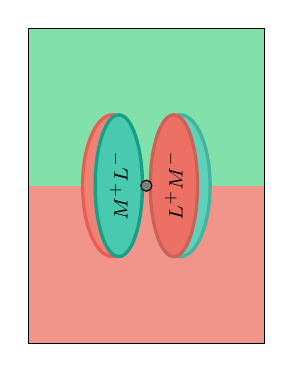
\begin{tikzpicture}
            \fill[emerald!60]                                             (-1.50, 2.00) rectangle (1.50, 0.00);
            \fill[alizarin!60]                                            (-1.50,-2.00) rectangle (1.50, 0.00);
            \filldraw[greensea!80,    fill=turquoise!70, very thick]( 0.43, 0.00) ellipse   (0.38 and 0.90);
            \filldraw[color=alizarin!90,    fill=alizarin!70,  very thick](-0.43, 0.00) ellipse   (0.38 and 0.90);
            \filldraw[pomegranate!80, fill=alizarin!80,  very thick]( 0.35, 0.00) ellipse   (0.30 and 0.90)
                 node[color=black, anchor=center, rotate=90] {$\scriptstyle L^+M^-$};
            \filldraw[greensea,       fill=turquoise!80, very thick](-0.35, 0.00) ellipse   (0.30 and 0.90)
                 node[color=black, anchor=center, rotate=90] {$\scriptstyle M^+L^-$};
            \filldraw[color=black,          fill=gray]                    ( 0.00, 0.00) circle    (2pt);
            \draw (current bounding box.north east) rectangle (current bounding box.south west);
            \end{tikzpicture}
        \caption{Minimal Response}
    \end{subfigure}%
    \begin{subfigure}{0.2\textwidth}
        \centering
            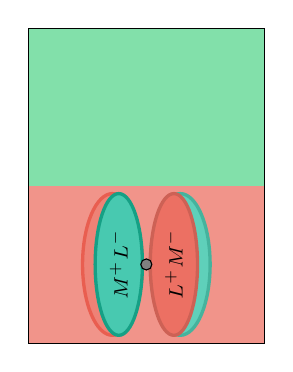
\begin{tikzpicture}
            \fill[emerald!60]                                             (-1.50, 2.00) rectangle (1.50, 0.00);
            \fill[alizarin!60]                                            (-1.50,-2.00) rectangle (1.50, 0.00);
            \filldraw[greensea!80,    fill=turquoise!70, very thick]( 0.43,-1.00) ellipse   (0.38 and 0.90);
            \filldraw[color=alizarin!90,    fill=alizarin!70,  very thick](-0.43,-1.00) ellipse   (0.38 and 0.90);
            \filldraw[pomegranate!80, fill=alizarin!80,  very thick]( 0.35,-1.00) ellipse   (0.30 and 0.90)
                 node[color=black, anchor=center, rotate=90] {$\scriptstyle L^+M^-$};
            \filldraw[greensea,       fill=turquoise!80, very thick](-0.35,-1.00) ellipse   (0.30 and 0.90)
                 node[color=black, anchor=center, rotate=90] {$\scriptstyle M^+L^-$};
            \filldraw[color=black,          fill=gray]                    ( 0.00,-1.00) circle    (2pt);
            \draw (current bounding box.north east) rectangle (current bounding box.south west);
            \end{tikzpicture}
        \caption{Minor Response}
    \end{subfigure}
    \caption{A double-opponent cell selective to vertically oriented borders with red to the right and green on the left; completely unresponsive to a horizontal border. While its $L^+$ receptive field might be strongly stimulated in (a) and (f), it's $L^-$ receptive field cancels it out. Similarly, in (c) and (d) its $M^+$ receptive field is stimulated but cancelled out by activity in its $M^-$ receptive field. In (b) and (e) both of its $L^+$ and $M^+$ receptive fields are moderately activated, but again, cancelled out by activation in its $L^-$ and $M^-$ receptive fields, respectively.}
\end{figure}

\end{document}